\documentclass[  11pt]{article}
\usepackage{graphicx, ulem}
\usepackage{amsthm}
\usepackage{amsmath}
\usepackage{listings}
 \usepackage{bookmark}
\usepackage{algorithm}
\usepackage{algpseudocode}
\usepackage{amsfonts,amssymb}
 \usepackage{enumerate} 
 
 \usepackage{tikz} %draw transition diagram 
\usetikzlibrary{arrows}%draw transition diagram 

 
\usepackage{color}

\definecolor{dkgreen}{rgb}{0,0.6,0}
\definecolor{gray}{rgb}{0.5,0.5,0.5}
\definecolor{mauve}{rgb}{0.58,0,0.82}
 
\newcommand*{\rom}[1]{\expandafter\@slowromancap\romannumeral #1@}

\lstset{frame=tb,
  language=Matlab,
  aboveskip=3mm,
  belowskip=3mm,
  showstringspaces=false,
  columns=flexible,
  basicstyle={\small\ttfamily},
  numbers=none,
  numberstyle=\tiny\color{gray},
  keywordstyle=\color{blue},
  commentstyle=\color{dkgreen},
  stringstyle=\color{mauve},
  breaklines=true,
  breakatwhitespace=true
  tabsize=3
}


% ********************** ********************** **********************
%\usepackage[lastexercise]{exercise}
\usepackage[lastexercise,noanswer]{exercise}
%		use this command to hide/not-hide answers
% ********************** ********************** **********************
% ********************** ********************** **********************

% 
%\newcounter{Problem}
%\newenvironment{Problem}{\begin{Exercise}[name={Problem},
%counter={Problem}]}
%{\end{Exercise}}
%\newcommand{\bp}{\begin{Problem}}
%\newcommand{\ep}{\end{Problem}}
%
%\renewcounter{Problem}[section]

%
%\usepackage[nosolutionfiles]{answers}
%\Newassociation{sol}{Solution}{ans}
%

\newcommand{\hws}{ {\underline{\tt Homework$\star$}} }
\newcommand{\optional}{ {\it optional} }


%probability 
\newcommand{\p}{ {\Pr}}
\newcommand{\prob}{{\Pr}}
\newcommand{\PP}{\mbox{PP}}
%condition prob
\newcommand{\cPr}[2]{{\Pr\left(#1\mid #2\right)}}

\newcommand{\FF}{{\mathbb{F}}}
\newcommand{\Exp}{\mbox{Exp}}
\newcommand{\Poi}{\mbox{Poi}}
\newcommand{\Bin}{\mbox{Bin}}

\newcommand{\e}{ \operatorname{E}}
\newcommand{\Var}{\operatorname{var}}
\newcommand{\Std}{\operatorname{std}}

%Matrix  %mathbf
\newcommand{\Pm}{{\mathbf{P}}}
\newcommand{\Qm}{{\mathbf{Q}}}
\newcommand{\Mm}{{\mathbf{M}}}

\newcommand{\eye}{{\mathbf{I}}}
\newcommand{\onem}{{\mathbb{1}}}
\newcommand{\ii}{\mathbf{i}}
%imaginary symbol


\newcommand{\la}{\lambda}

%State number 
\newcommand{\snum}[1]{ \raisebox{.5pt}{\textcircled{\raisebox{-.9pt} {#1}}}}
  
%real number
\newcommand{\Real}{{\mathbb{R}}}
%integer 
\newcommand{\ZZ}{\mathbb{Z}}
%positive integer 
\newcommand{\NN}{\mathbb{N}}



\newcommand{\inpd}[2]{\left\langle #1, #2 \right\rangle}
\newcommand{\abs}[1]{\left\vert#1\right\vert}
\newcommand{\norm}[1]{\left\|#1\right\|}


\newcommand{\set}[1]{\left\{#1\right\}}


\newcommand{\Xnn}{X_{n+1}}
\newcommand{\Xn}{X_{n}}

\newcommand{\MC}{Markov Chain}

\newcommand{\tm}{transition matrix}
\newcommand{\rv}{random variable}


\newcommand{\po}{Poisson }
\newcommand{\pp}{Poisson process }



\newcommand{\ie}{{\it{i.e.}}}



\newcommand{\transpose}{\textsf{T}} % or, \intercal
\newcommand{\tr}{{\textsf{T}}}
\newcommand{\rt}{{\textbf{r}}}



\def\biz{\begin{itemize} }
\def\eiz{\end{itemize}}



 \def\ben{\begin{enumerate}}
\def\een{\end{enumerate}}

  


\newcommand{\hb}[1]{ {\color{blue}{#1} }}

  



\begin{document}

\title{ Solution  Manual  of MA4546}

 
%\address{Xiang ZHOU, Department of  Math,City University of Hong Kong, Hong Kong SAR }


%\date{2015-2016 Sem A}
\maketitle

 This solution manual   includes more   exercises  than the assigned homework.


\section*{Chapter 1}
\begin{ExerciseList}
\Exercise
 A pairwise independent collection of random variables is a set of random variables
any two of which are independent. Any collection of mutually independent
random variables is pairwise independent, but some pairwise independent
collections are not mutually independent. Consider the following example.
Toss a fair coin two times. Define the following events
\begin{itemize}
\item A: head appears on the first toss
\item B: head appears on the second toss
\item C: both tosses yield the same outcome.
\end{itemize}
Are the events A,B and C mutually independent ? Are they pairwise independent?
 
\Answer
It is easy to find out that:
$P(A)=P(B)=P(C)=\frac{1}{2}$; $P(A\cap B) = P(A\cap C) = P(B\cap C) = \frac{1}{4}$; and $P(A\cap B\cap C) = \frac{1}{4}$. \\

So $A, B, C$ are pairwise independent because $P(A\cap B) = P(A)P(B)$; $P(A\cap C) = P(A)P(C)$; $P(B\cap C) = P(B)P(C)$. But they are not mutually independent because $P(A\cap B\cap C) \neq P(A)P(B)P(C)$. (Refer to page 15 in the slide for the definition.)\\


\Exercise[difficulty=4]
 If $p$ and $q$ are two pdfs defined on $\Real$, prove that the Kullback-Leibler
divergence (or "relative entropy") of $q$ from $p$, which is defined as
$$D(p\|q)=\int p(x)\log\frac{p(x)}{q(x)}$$
is always non-negative.

\Answer
$\varphi(x)=-\log(x)$ is a convex function.
According to Jensen's inequality,
$$\mathbb{E}[\varphi(\frac{q(x)}{p(x)})] \geq \varphi (\mathbb{E}[\frac{q(x)}{p(x)}])$$
Thus we have
\[
\begin{split}
D(p\|q) &=\int p(x)\log(\frac{p(x)}{q(x)})dx\\
&=\int -p(x) \log(\frac{q(x)}{p(x)})dx\\
&=\mathbb{E}_p[\varphi(\frac{q(x)}{p(x)})]\\
&\geq \varphi (\mathbb{E}_p[\frac{q(x)}{p(x)}])\\
&=-\log(\int\frac{q(x)}{p(x)}p(x)dx)\\
&=-\log(\int q(x)dx)\\
&=-\log1\\
&=0
\end{split}
\]


\Exercise
 If  two r.v.s X and Y are independent, then
\[
p_{X|Y}(x|y)=p_X(x), \mathbb{E}(X|Y)=\mathbb{E}(X)
\]

\Answer 
$$p_{X|Y}(x|y)=\frac{p_{X,Y}(x,y)}{p_Y(y)}=\frac{p_{X}(x)p_Y(y)}{p_Y(y)}=p_X(x)$$
$$\mathbb{E}[X|Y]=\int xp_{X|Y}(x|y)dx=\int xp_X(x)dx= \mathbb{E}(X)$$

\Exercise
If $\{X_1, X_2,.., X_n \}$ is mutually independent, then $\Var(\sum_iX_i)=\sum_i \Var(X_i)$

\Answer
If $\{X_1,X_2,..,X_n \}$ is mutually independent, then $\mathbb{E}[X_i X_j]=\mathbb{E}[X_i]\mathbb{E}[X_j]$ for all $i,j, i\neq j$.
\[
\begin{split}
var(\sum_i{X_i})
&=\mathbb{E}[(\sum_i{X_i})^2]-(\mathbb{E}[\sum_i X_i])^2\\
&=\mathbb{E}[\sum_i X_i^2+2\sum_{i<j}X_iX_j]-(\sum_i \mathbb{E}[X_i])^2\\
&=\sum_i \mathbb{E}[X_i^2]+2\sum_{i<j}\mathbb{E}[X_iX_j]-\sum_i (\mathbb{E}[X_i])^2-2\sum_{i<j}\mathbb{E}[X_i]\mathbb{E}[X_j]\\
&=\sum_i \mathbb{E}[X_i^2]-\sum_i (\mathbb{E}[X_i])^2\\
&=\sum_i var(X_i)\\
\end{split}
\]

\Exercise 

Suppose that $X=(X_1, X_2)$ is a two dimensional Gaussian random variable with mean $\mu=(\mu_1, \mu_2) $ and the covariance matrix $\Sigma=\left(
  \begin{array}{cc}
    \sigma_1^2 & \rho\sigma_1\sigma_2  \\
    \rho\sigma_1\sigma_2 & \sigma_2^2 \\
  \end{array}
\right) $. What is the conditional pdf $p(x_1|x_2)$ of $X_1$ given $X_2=x_2$? For what value of $\rho$, $X_1$
and $X_2$ are independent? Verify the variance decomposition theorem for this two Gaussian variables $X_1$ and $X_2$.

\Answer

\textrm{(i)}\[
\begin{split}
p(x_1|x_2)&=\frac{p(x_1,x_2)}{p(x_2)}\\
&=\frac{1}{\sqrt{2\pi}\sigma_1\sqrt{1-\rho^2}}\exp\{-\frac{1}{2(1-\rho^2)}[\frac{(x_1-\mu_1)^2}{\sigma_1^2}-2\rho(\frac{x_1-\mu_1}{\sigma_1})(\frac{x_2-\mu_2}{\sigma_2})+\frac{\rho^2(x_2-\mu_2)^2}{\sigma_2^2}]\}\\
&=\frac{1}{\sqrt{2\pi}\sigma_1\sqrt{1-\rho^2}}\exp\{-\frac{[x_1-(\mu_1+\rho\frac{\sigma_1}{\sigma_2}(x_2-\mu_2))]^2}{2\sigma_1^2(1-\rho^2)}\}
\end{split}\]
\[
X_1|_{X_2=x_2}\sim N(\mu_1+\rho\frac{\sigma_1}{\sigma_2}(x_2-\mu_2), \sigma_1^2(1-\rho^2))
\]
%$$\sigma_1^2=var(X_1)=E(X_1^2)-[E(X_1)]^2=E(X_1^2)-\mu_1^2$$
%$$\sigma_2^2=var(X_2)=E(X_2^2)-[E(X_2)]^2=E(X_2^2)-\mu_2^2$$
\textrm{(ii)}%$$\rho\sigma_1\sigma_2=cov(X_1,X_2)=E(X_1X_2)-[E(X_1)E(X_2)]^2=E(X_1X_2)-\mu_1\mu_2$$
%$$\mu_1\mu_2=E(X_1)E(X_2)=E(X_1X_2)=\rho\sigma_1\sigma_2+\mu_1\mu_2$$
For $\rho=0$, we   see
\[
\begin{split}
p(x_1,x_2)&=\frac{1}{2\pi\sigma_1\sigma_2}\exp\{-\frac{1}{2}[\frac{(x_1-\mu_1)^2}{\sigma_1^2}+\frac{(x_2-\mu_2)^2}{\sigma_2^2}]\}\\
&=\frac{1}{\sqrt{2\pi}\sigma_1}\exp\{-\frac{(x_1-\mu_1)^2}{2\sigma_1^2}\}\frac{1}{\sqrt{2\pi}\sigma_2}\exp\{-\frac{(x_2-\mu_2)^2}{2\sigma_2^2}\}\\
&=p(x_1)p(x_2)
\end{split}
\]
Then 
$X_1$ and $X_2$ are independent.\par
\textrm{(iii)}
\[
\mathbb{E}(X_1|X_2)=\mu_1+\rho\frac{\sigma_1}{\sigma_2}(X_2-\mu_2)
\]
\[
var(X_1|X_2)=\sigma_1^2(1-\rho^2)
\]
\[
var(X_1)=\sigma_1^2,\ var(X_2)=\sigma_2^2
\]
It is easy to show that $var(X_1)=\mathbb{E}[var(X_1|X_2)]+var[\mathbb{E}(X_1|X_2)]$.

\Exercise
 Find the moment-generating and characteristic functions
for the following distributions:
Bernoulli distribution $\mathsf{Bern}(p)$, Poisson distribution $\mathsf{Poi}(\lambda)$, 
exponential distribution $\mathsf{Exp}(\lambda)$,  normal distribution $N(\mu,\sigma^2)$.


\Answer 
\begin{enumerate}
\item Bernoulli distribution: $\Pr(X=1)=p=1-\Pr(X=0)$
\[M(t)=\e[e^{t X}] = 1-p + pe^t, ~~\varphi(t)= \e[e^{\ii t X}]= 1-p + pe^{\ii t} \]
\item  Poisson distribution $\mathsf{Poi}(\lambda)$:
$\Pr(X=k)=e^{-\lambda }  \lambda^k / k!$.
\[M(t)=\e[e^{t X}] = \sum_{k\geq 0} e^{tk} e^{-\lambda }  \lambda^k / k!
=   e^{-\lambda }   \sum_{k\geq 0}  (e^t \lambda) ^k / k! 
=\exp\left(  \lambda (e^t -1) \right) ,\]
\[
\varphi(t)= \e[e^{\ii t X}]= \exp\left(  \lambda (e^{\ii t} -1) \right).\]
\item 
exponential distribution $\mathsf{Exp}(\lambda)$:
$ p(x)=\lambda e^{-\lambda x}, ~~x>0$.
\[M(t)=\e[e^{t X}]  = \int_0^{+\infty}   \lambda e^{-(\lambda-t) x} dx
=  1 /(1-t/\lambda) \mbox{ if } t < \lambda. \]
\[
\varphi(t)= \e[e^{\ii t X}]=1 /(1-\ii t/\lambda) , ~~\forall t\in \Real.
\]
\item We give the result for the Normal distribution in any $d\geq 1$ dimension.
So the $\Real^d$-valued random variable  $\vec{X}\sim \mathcal{N}(\vec{\mu}, \Sigma)$ with the mean $\e \vec{X}=\vec{\mu}\in \Real^d$
and the covariance matrix $\Sigma \in \Real^{d\times d}$ whose $i,j$ entry is
 $\e((X_i-\mu_i)( X_j-\mu_j))$. Then the pdf is 
$$p(\vec{x})= \frac{1}{(2\pi)^{d/2}\sqrt{\det{\Sigma}}}\exp\left \{  - (\vec{x}-\vec{\mu})^\tr \Sigma^{-1}  (\vec{x}-\vec{\mu})/2\right\}.$$

The moment-generation function is defined over a vector-valued variable $\vec{t}\in\Real^d$:
\[
\begin{split}
M(\vec{t})
&= \e e^{\vec{t} \cdot \vec{X}}
\\
&= \int_{\Real^d} 
\frac{1}{(2\pi)^{d/2}\sqrt{\det{\Sigma}}}
\exp\left(  - (\vec{x}-\vec{\mu})^\tr \Sigma^{-1}  (\vec{x}-\vec{\mu})/2
+\vec{t} \cdot \vec{x}\right)  d \vec{x}
\\
&=e^{\vec{t} \cdot \vec{\mu}} \int_{\Real^d} 
\frac{1}{(2\pi)^{d/2}\sqrt{\det{\Sigma}}}
\exp\left(  - \vec{y}^\tr \Sigma^{-1}\vec{y}/2
+\vec{t}\cdot \vec{y}\right)  d \vec{y}
\\
&=
e^{\vec{t} \cdot \vec{\mu}} \int_{\Real^d} 
\frac{1}{(2\pi)^{d/2}\sqrt{\det{\Sigma}}}
\exp\left(  - (\vec{y}-\Sigma \vec{t})^\tr \Sigma^{-1}(\vec{y}-\Sigma \vec{t})/2
+\vec{t}^\tr \Sigma \vec{t}/2\right)  d \vec{y}
\\
&=e^{\vec{t} \cdot \vec{\mu}+\vec{t}^\tr \Sigma \vec{t}/2 } \int_{\Real^d} 
\frac{1}{(2\pi)^{d/2}\sqrt{\det{\Sigma}}}
\exp\left(  - (\vec{z} )^\tr \Sigma^{-1}(\vec{z} )/2
 \right)  d \vec{z}
 \\
 &=\exp\left( \vec{t} \cdot \vec{\mu}+ \frac12 \vec{t}\cdot \Sigma \vec{t}   \right)
 \\
 &=\exp\left( \sum_{i=1}^dt_i \mu_i + \frac12 \sum_{i=1}^d\sum_{j=1}^d t_i \Sigma_{ij}t_j\right)
\end{split}.
\]
The characteristic function is 
\[
\varphi(t) = M(\ii \vec{t})= \e e^{\ii \vec{t} \cdot \vec{X}}=
\exp\left( \ii \vec{t} \cdot \vec{\mu}- \frac12 \vec{t}\cdot \Sigma \vec{t}   \right).
\]
\end{enumerate}

 

\Exercise[difficulty=5]

Show that 
\[\e [ |X-h(Y)|^2] =\min_{g \mbox{ is a function }}  \e (  |X-g(Y)|^2    ) \]
where the function  $h(y)$ is the conditional expectation  $h(y)=\e(X|Y=y)$.

\Answer
We show first that   $\e[(X-h(Y) )  f(Y) ]=0$ is true  for any function $f$.
Using the double expectation theorem, we have 
\[
\begin{split}
&\e[(X-h(Y) )  f(Y) ] = \e ( \e[(X-h(Y) )  f(Y) | Y  ]  )\\
=& \e ( \e(Xf(Y)|Y) -h(Y)   f(Y))   \\
= &\e ( f(Y) \e(X|Y))  -\e(h(Y)   f(Y)   )\\
=&0.
\end{split}
\]


 Then use the triangular equality
$(x-g)^2=(x-h)^2+(g-h)^2-2(x-h)(g-h)$and let $f=g-h$,
\[\e (  |X-g(Y)|^2    )
=\e (  |X-h(Y)|^2   ) + \e(g(Y)-h(Y))^2,\]
from which the conclusion is straightforward.



\Exercise[name =\optional]
Show that if $(X_t)$ is a martingale, then 
its expectation $\e(X_t)$ is independent of time $t$. 
\Answer
Since $\e(X_t|X_s) = X_s$ for all $s\leq t$. then
$\e(\e(X_t|X_s))=\e(X_s)$. By the double expectation theorem, 
$\e(X_t)=\e(X_s)\equiv \e(X_0)$.

\Exercise [name=\optional, difficulty=4]
 For the random walk  $(X_n=\sum_{i=1}^n Z_n)$
 where $\p(Z_n=1)=p$ and $\p(Z_n=-1)=q=1-p$, find the value 
of a positive number $\sigma$
such that $Y_n:=(X_n-\mu n)^2 -\sigma^2 n $ is a martingale,
where $\mu=\e Z_n =p-q$.
\Answer
Since $Y_n$ is a margingale, then
$\e Y_n=\e Y_0=0$. So,
$n \sigma^2 = \e (X_n-\mu n)^2= \e (\sum_{i=1}^n  (Z_i - \e Z_i))^2
=\Var(\sum_{i=1}^n Z_i)=\sum_i \Var(Z_i)=
(1-\mu^2)n$.
So, $\sigma=\sqrt{1-\mu^2}=2\sqrt{pq}$, which is the standard deviation of 
$Z_i$.

Next we we need show that $Y_n$ is indeed a martingale for such a 
$\sigma=\sqrt{1-\mu^2}$.
Without loss of generality we assume $p=q=1/2$ (otherwise, consider $\widetilde{X}_n:=X_n-\mu n$), then $\mu=0,\sigma=1$.
$Y_n=X_n^2-n$. Note that $Y_{n+1}=Y_n + Z_{n+1}^2 + 2 X_n Z_{n+1}-1$.
We have 
\[\e (Y_{n+1} \mid Y_n)=Y_n+ \e(Z_{n+1}^2\mid Y_n) + X_n \e(Z_{n+1}\mid Y_n) -1
=Y_n.\]


\end{ExerciseList}

\newpage
\section*{Chapter 2 (part i)}
\setcounter{Exercise}{0}
\begin{ExerciseList}


 \Exercise
 Let $X_n$  be the random walk on $S=\ZZ$
($X_0=0$) with transition probability
$\p(X_{n+1}=i+1\mid X_n) = p$
and $\p(X_{n+1}=i-1\mid X_n) = q=1-p$.

Calculate the mean $\e X_n$, the variance $\Var{X_n}$
and the autocovariance 
$c(n,m):=\e[(X_n - \e X_n)(X_m - \e X_m)]$.
%answer 0, 4pq, \min(n,m)4pq.

\Answer
$\e X_n = n\mu$ where $\mu=p-q$.\par
$\Var X_n = \sum_i \Var Z_i = 4npq$. \par
Assume that $m<n$, then  let $k=n-m$,
so.
\[\begin{split}
c(n,m)&=
\e\left[(X_{m}  -m\mu)^2 + \sum_{i=m+1}^{n}( Z_i - \mu)(X_m - m\mu)\right] \\
&=\Var(X_m) + \e\left[ \sum_{i=m+1}^{n} (Z_i - \mu)(X_m - m\mu)\right] 
\\
&=
\Var(X_m) +\sum_{i=m+1}^{n}  \e ( Z_i - \mu) \cdot \e (X_m - m\mu) 
\\
&=\Var(X_m)\\
 &= 4mpq \\&= 4pq \min(m,n).
\end{split}
\]

\Exercise[difficulty=4]

 Assume that $\{X_n\}$, $n=1,2,\cdots,$ are iid  $\{-1,1\}$-valued random variables.
 $\mathbb{P}(X_i=1)=p$ and $\mathbb{P}(X_i=-1)=1-p$.   For any $n\geq 1$,  define new random variables 
 \[ 
 S_n = \sum_{i=0}^n X_i, \
   Y_n = X_{n}+X_{n-1}, 
 \]
and the two-dim random vector
   $
        Z_n = \begin{bmatrix} X_{n-1} \\ X_n\end{bmatrix}
   $.
Discuss if  the  stochastic processes $\{S_n\}$,  $\{Y_n\}$,  $\{Z_n\}$ are Markov chains. Why? Write the corresponding transition matrices for Markov chains. \\

\Answer

Recall that   the definition of Markov Chain $\{X_n\}$ is given as follows:
\[
\mathbb{P}(X_{n+1}=j\:\vert X_{n}=i,\, X_{n-1},\ldots X_{0})= \mathbb{P}(X_{n+1}=j\:\vert X_{n}=i)
\qquad (*)
\]
$\forall i, j \in S$ . We discuss this property for $S_n, Y_n$ and $Z_n$ respectively.
\begin{itemize}
\item  $\{S_n\}$ is actually an 1D random walk. It is a Markov chain.

 $\mathbb{P}(S_{n+1} = j | S_n = i, S_{n-1}, ..., S_0) = \mathbb{P}(S_n + X_{n+1} = j | S_n = i, S_{n-1}, ..., S_0) = \mathbb{P}(X_{n+1} = j-S_n | S_n = i, S_{n-1}, ..., S_0)$. 
 Note $S_n-S_{n-1}=X_n$, then
the conditional information of $S_n = i, S_{n-1}, ..., S_0$  is 
equal to the conditional information of $S_n = i, X_{n-1}, ..., X_1, X_0$.
 Since $\{X_n\}$ are iid,  meaning the choice of $X_{n+1}$ does not depend on $X_i$ $\forall i \in \{0,1,...,n\}$, $\mathbb{P}(X_{n+1} = j-S_n | S_n = i, S_{n-1}=s_{n-1}, ..., S_0=s_0) = \mathbb{P}(X_{n+1} = j-S_n | S_n = i,X_{n-1}=s_{n-1}-s_{n-2},\ldots, X_1=s_1-s_0, X_0=s_0)
 = \mathbb{P}(X_{n+1} = j-S_n | S_n = i)=
  \mathbb{P}(X_{n+1}=j-i) $. Hence $\{S_n\}_{n\ge 0}$ is a Markov Chain. \\ 

The value of $S_n$ ($n\in \mathbb{N}$) covers the whole $\mathbb{Z}$, so the state space for $S_n$ is $\mathbb{Z}$ (see page 7, part 1 of lecture slides) and the transition matrix is a countable infinite matrix with element 
\begin{equation}
\begin{array}{ll}
\mathbb{P}(i,j) = p & \text{ if } j = i+1 \\
\mathbb{P}(i,j) = 1 - p & \text{ if } j = i-1 \\
\mathbb{P}(i,j) = 0 & \text{ otherwise} \\
\end{array}
\end{equation}
Note that $P(i,j)$ means the probability of finding next step $S_{k+1}$ as $j$ provided that current value of $S_k$ is $i$ ($k\in \mathbb{N}$), and that $i,j\in \mathbb{Z}$.



 
\item The state space of $\{Y_n\}$ is $S=\{-2,0,2\}$.
We shall show that $\{Y_n\}$ is not  a Markov chain by constructing a counterexample  for  equation (*) .
Note that  the state space of $\{X_n\}$ is $\{1,-1\}$.
Thus, $\{Y_n=2\}=\{X_n=1, X_{n-1}=1\}$ and 
$\{Y_n=-2\}=\{X_n=-1, X_{n-1}=-1\}$ and 
$\{Y_n=0\}=\{X_n=-1, X_{n-1}=1\}\cup\{X_n=1, X_{n-1}=-1\} $. \par
We have the following calculation.
$\mathbb{P}(Y_{3} = 2 | Y_{2} = 0,  Y_{1}= 0 )
=\mathbb{P}(Y_{3} = 2 | Y_{2} = 0,  Y_{1}= 0, X_0=1 ) p + 
\mathbb{P}(Y_{3} = 2 | Y_{2} = 0,  Y_{1}= 0 , X_0=-1 ) (1-p)  
=\mathbb{P}(X_{3}=1,X_2 = 1 | X_{2} = 1,  X_{1}= -1, X_0=1 ) p + 
\mathbb{P}(X_{3} = 1, X_2=1 | X_{2} = -1,  X_{1}= 1 , X_0=-1 ) (1-p)  
=\mathbb{P}(X_{3}=1 ) p + 0 =p^2.
$

$\mathbb{P}(Y_{3} = 2 | Y_{2} = 0,  Y_{1}= 2 )
=\mathbb{P}(X_{3}=1,X_2 = 1 | Y_{2} = 0,  X_{1}= 1, X_0=1 )
=\mathbb{P}(X_{3}=1,X_2 = 1 | X_{2} = -1,  X_{1}= 1, X_0=1 )
=0 $.


$\mathbb{P}(Y_{3} = 2 | Y_{2} = 0,  Y_{1}= -2 )
=\mathbb{P}(X_{3}=1,X_2 = 1 | Y_{2} = 0,  X_{1}= -1, X_0=-1 )
=\mathbb{P}(X_{3}=1,X_2 = 1 | X_{2} = 1,  X_{1}= -1, X_0=-1 )
=p $.

Thus, the conditional probability $\mathbb{P}(Y_{n+1}|Y_{n}, \ldots, Y_1, Y_0)$
can not be determined by the conditional value of  $Y_n$.
$\{Y_n\}$ is not a Markov chain.

{\bf remark}: The trouble for   non-Markovian  comes from the case $\{Y_n=0\}$,
though we have the following result.

For any $n$ and a sequence $j,  i_{n-1},\ldots, i_1\in S$,
$\mathbb{P}(Y_{n+1} =j | Y_n = -2,  Y_{n-1}=i_{n-1}\ldots, Y_1=i_1) = \mathbb{P}(X_{n+1} =j-X_n | X_n=-1,X_{n-1}= -1,
X_{n-1}+X_{n-2}=i_{n-1},\ldots, X_1+X_0=i_1) =  
\mathbb{P}(X_{n+1} = j+1 | X_n=-1,X_{n-1}= -1,
X_{n-1}=i_{n-1}-X_{n-2},\ldots, X_1=i_1-X_0 ,X_0)
=\mathbb{P}(X_{n+1}=j+1)=
  \begin{cases}
p &\mbox{ if }  j=0;
\\  1-p& \mbox{ if }  j=-2; 
\\ 0 &\mbox{ if }  j=2
\end{cases} .$

Similarly, 
$\mathbb{P}(Y_{n+1} = j| Y_n = 2,  Y_{n-1}=i_{n-1}\ldots, Y_1=i_1) = \mathbb{P}(X_{n+1}=j-1)=
\begin{cases}
p &\mbox{ if }  j=2;
\\  1-p& \mbox{ if }  j=0; 
\\ 0 &\mbox{ if }  j=2.
\end{cases} $


 

\item $\{Z_{n}\}$ can be treated as   2D  points. \\

With the information of $Z_n$, the value of $X_n$ is known, and thus the first component  in $Z_{n+1} = \begin{bmatrix} X_{n} \\ X_{n+1}\end{bmatrix}$ is determined as well. $ \{X_n\}$ are iid $\Rightarrow \mathbb{P}(Z_{n+1} = \begin{bmatrix} j_1 \\ j_2 \end{bmatrix} | Z_{n} = \begin{bmatrix} i_1 \\ i_2\end{bmatrix}, Z_{n-1},...,Z_1) = \mathbb{P}(X_{n+1} = j_2) \delta(j_1,i_2)$ where $\delta(x,y)$ is a delta function with value 1 if $x=y$, and with value 0 if $x\neq y$.\\

What's more, $\mathbb{P}(Z_{n+1} = \begin{bmatrix} j_1 \\ j_2 \end{bmatrix} |Z_{n} = \begin{bmatrix} i_1 \\ i_2\end{bmatrix}) = \mathbb{P}(X_{n+1} = j_2) \delta(j_1,i_2)$ as well. Hence $\{Z_n\}$ is indeed a Markov Chain. \\

The state space $\mathbb{S} = \{s_1 = \begin{bmatrix} -1 \\ -1\end{bmatrix}, s_2 = \begin{bmatrix} -1 \\ 1\end{bmatrix}, s_3 = \begin{bmatrix} 1 \\ -1\end{bmatrix}, s_4 = \begin{bmatrix} 1 \\ 1\end{bmatrix}\}$.

The transition matrix is therefore $P = \begin{bmatrix}
1-p & p & 0 & 0 \\
0 & 0 & 1-p & p \\
1-p & p & 0 & 0 \\
0 & 0 & 1-p & p \\
\end{bmatrix}$ where $P_{ij}$ ($i,j\in\{1,2,3,4\}$) means the probability of finding $Z_{k+1} = s_j$ provided that $Z_{k} = s_i$.\\
 
  
 \end{itemize}


\Exercise[origin={textbook p51, 2.13}]  Consider the following weather model. The weather normally behaves as in
Example 2.3. However, when the cloudy spell lasts for two or more days, it continues to be cloudy for another day with probability .8 or turns rainy with probability .2. Develop a four-state DTMC model to describe this behaviour.\\

\Answer 
Denote the weather on day $n$ by $\set{W_n}$ taking values in    $\set{s, c, r }$.
Then the extra condition is $\p(W_{n+1} =c \vert W_{n} =W_{n-1}=c)=0.8$
and $\p(W_{n+1} = r \vert W_{n} =W_{n-1}=c)=0.2$,
$\p(W_{n+1} =s \vert W_{n} =W_{n-1}=c)=0$.
However, 
the probability $ \p(W_{n+1}   \vert W_{n} =c, W_{n-1}\neq c)$
 will follow the original transition matrix, i.e.,
 $ \p(W_{n+1}=s   \vert W_{n} =c, W_{n-1}\neq c)=0.5$,
 $ \p(W_{n+1}=c   \vert W_{n} =c, W_{n-1}\neq c)=0.2$,
 $ \p(W_{n+1}=r   \vert W_{n} =c, W_{n-1}\neq c)=0.3$.
Apparently, the process $\set{W_n}$ is not a DTMC any more
since the information $W_{n-1}$ affects the   probability of $W_{n+1}$. 
\par


We need to handle the special case of two successive cloudy days by splitting the original 
 ``cloudy" state in Example 2.3 into two states.
Let $X_n$ be the weather conditions in Heavenly, defined as follows:
\[
X_n= 
\begin{cases}
1&  \mbox{if\ it\ is\ sunny\ on\ day\ } n,\\
2&  \mbox{if\ it\ is\ cloudy\ on\ day\ } n,\mbox{\ not\ cloudy\ on\ day\ } n-1\\
3& \mbox{if\ it\ is\ rainy\ on\ day\ }n\\
4&   \mbox{if\ it\ is\ both\ cloudy\ on\ day\ }n\ \&\ n-1
\end{cases}
\]

Then $X_n=4$ means $W_n=W_{n-1}=c$
and $X_n=2$ means $W_n=c, W_{n-1}\neq c$.

\bigskip
It is easy to verify that  $\p(X_n=i|X_{n-1},X_{n-2},...,X_{0})=\p(X_n=i|X_{n-1})$ holds for all $i$. We   model $X_n$ as a DTMC with transition matrix $\Pm$.
\[
\Pm=\left(\begin{array}{cccc}
     0.5 & 0.3 & 0.2 & 0 \\
     0.5 &  0  & 0.3 & 0.2 \\
     0.4 & 0.5 & 0.1 & 0 \\
     0   & 0   & 0.2 & 0.8 \\
  \end{array}\right).
\]
Note that if today is cloudy, tomorrow will have 0.2 probability to be cloudy again,
so $X_{n+1}$ goes to state 4. 

\bigskip

{\bf Remark:} If we do not impose the extra condition, and we simply split 
one state $c$ into two state $2$ and $4$ here. We have the following transition matrix for $\set{X_n}$:

\[
 \left(\begin{array}{cccc}
     0.5 & 0.3 & 0.2 & 0 \\
     0.5 &  0  & 0.3 & 0.2 \\
     0.4 & 0.5 & 0.1 & 0 \\
     0.5   & 0   & 0.3 & 0.2 \\
  \end{array}\right).
\]
Note that the second row equals  the fourth row in this matrix (the similar conclusion holds in general).

\Exercise[origin={p51. 2.16}]
A total of $N$ balls are put in two urns, so that initially urn A has $i$ balls and
urn B has $N-i$ balls. At each step, one ball is chosen at random from the $N$ balls.
If it is from urn A, it is moved to urn B, and vice versa. Let $X_n$ be the number
of balls in urn A after $n$ steps. Show that $\{X_n, n\geq0\}$ is a DTMC, assuming that
the successive random drawings of the balls are independent. Display the transition
probability matrix of the DTMC.\\

\Answer
\[
X_n=
\begin{cases}
X_{n-1}-1 &\mbox{ if\ one\ ball\ is\ chosen\ from\ urn\ A}\\
X_{n-1}+1& \mbox{ if\ one\ ball\ is\ chosen\ from\ urn\ B}
\end{cases}
\]
$$P(X_n=X_{n-1}-1)=\frac{X_{n-1}}{N},~~~ P(X_n=X_{n-1}+1)=\frac{N-X_{n-1}}{N}$$
Since each draw of ball is independent, $P(X_n=i|X_{n-1}, ...X_1)=P(X_n=i|X_{n-1})$, thus $\{X_n, n\geq0\}$ is a DTMC.\\

There are $N+1$ states for $X_n$, $S=(0, 1,2,...,N)$
\[
P=\left(\begin{array}{ccccccccc}
     0           & 1   & 0             & 0 & 0             & ... &0& 0 & 0\\
     1/N &  0  & (N-1)/N & 0 & 0             & ...&0 & 0 & 0\\
     0           & 2/N & 0 & (N-2)/N & 0 & ... &0& 0 & 0\\
     \vdots       & \vdots&\vdots& \vdots&\vdots &\vdots & \vdots&\vdots & \vdots\\
     0            &     0   & 0 & 0 &0& ... & (N-1)/N &0 & 1/N\\
     0            &     0   & 0 & 0 & 0&... & 0 &1 & 0\\
  \end{array}\right)
\]
Note that here the boundary condition is of the type ``reflection".

\Exercise[origin={p53,2.10}]
Consider the weather model of Example 2.3. Compute the probability that
once the weather becomes sunny, the sunny spell lasts for at least 3 days.

\Answer
Define the event $A$: once the weather becomes sunny, the sunny spell lasts for at least 3 days\\
\[
\begin{split}
P(A)&=P(X_{n+2}=1, X_{n+1}=1|X_n=1)\\
&=P(X_{n+2}=1|X_{n+1}=1, X_n=1)P(X_{n+1}=1|X_n=1)\\
&=P(X_{n+2}=1|X_{n+1}=1)P(X_{n+1}=1|X_n=1)\\
&=0.5^2=0.25.
\end{split}
\]
 



\Exercise[origin={p53, 2.11}]
Compute the expected length of a rainy spell in the weather model of Example
2.3.\\
\Answer
Define the event $A_n$: the rainy spell lasts for $n$ days. The previous problem shows that 
$P(A_n)  =(1-p_{33})(p_{33})^{n-1}=0.9(0.1)^{n-1}$. So the expected length of a rainy spell is 
\[\begin{split}
\sum_{n=1}^\infty nP(A_n) & = \sum_{n\ge 1} n \times 0.9 \times (0.1)^{n-1}\\
& =0.9(1+2\times0.1+3(0.1)^2+4(0.1)^3+......)=\frac{10}{9}.
\end{split}\]
Note: for $x\in (0,1)$, we have $\sum_{n\ge 1}^{\infty} n x^{n-1} = (\sum_{n\ge 1} x^n)^{'} = (\frac{x}{1-x})^{'} = \frac{1}{(1-x)^2}$. 
 



\Exercise[origin={p53-54, 2.15b}]
Compute the occupancy matrix M(10) for the DTMCs with transition matrices
as given below:
\[
P=\left(\begin{array}{cccc}
   0&1&0 &0\\
   0&0&1&0\\
   0&0&0&1\\
   1&0&0&0\\
 \end{array}\right)
\]
\Answer
\[
M(10)=\sum_{t=0}^{10}P^t
\]
\[P^0=P^4=P^8=I, \text{ } P^1=P^5=P^9=P\],
\[
P^2=P^6=P^{10}=\left(\begin{array}{cccc}
   0&0&1&0\\
   0&0&0&1\\
   1&0&0&0\\
   0&1&0&0\\
 \end{array}\right)
\]
\[
P^3=P^7=\left(\begin{array}{cccc}
   0&0&0&1\\
   1&0&0&0\\
   0&1&0&0\\
   0&0&1&0\\
 \end{array}\right)
\]
\[
M(10)=\sum_{t=0}^{10}P^t=\left(\begin{array}{cccc}
   3&3&3&2\\
   2&3&3&3\\
   3&2&3&3\\
   3&3&2&3\\
 \end{array}\right)
\]

MATLAB code is as follows
\begin{lstlisting}
EDU>> P = [0 1 0 0; 0 0 1 0; 0 0 0 1; 1 0 0 0];
EDU>> M = zeros(4,4);
EDU>> for i = 0:10
M = M+P^i;
end
EDU>> disp(M)
     3     3     3     2
     2     3     3     3
     3     2     3     3
     3     3     2     3
\end{lstlisting}


\end{ExerciseList}


\newpage
\section*{Chapter 2 (part ii, part iii)}
\setcounter{Exercise}{0}

\begin{ExerciseList}

\Exercise 
 Consider the two-state DTMC with the transition matrix 
 $$P = \begin{bmatrix} 1- a & a \\ b & 1-b \end{bmatrix}$$
$a,b\in [0,1]$. 
Discuss the reducibility, periodicity and limiting/stationary/occupancy distributions
to classify the DTMC for different $a$, $b$.



\Answer
\begin{enumerate}
\item  
$a=b=0$ (both $a$ and $b$ are zeros).
\[
P=\left(\begin{array}{cc}
1 &0\\
0 &1\\
\end{array}\right)
\]
In this DTMC, state 1 can only communicate with state 1   and state 2 can only communicate with state 2 but 
there is no communication between these two states. Thus   it's reducible. \par
Its  limiting distribution is not unique since $\lim_n P^n=P$ does not have the same row.
In fact $a^{(n)}=a^{(0)}$, which strongly depends on the initial law $a^{(0)}$.
\par
For any stochastic vector $\mu$, $\mu=\mu P$ holds. Thus any initial distribution $\mu$ is a stationary distribution of this DTMC.\par
Its occupancy distribution  is also not unique   for the same reason
that  $\frac{M(n)}{n+1}\equiv P$ since $P^n \equiv P$ for any $n$.

\par

\item 
$a+b>0$, $ab=0$ (i.e.,  either $a$ or $b$ is zero, but not both).\par
For $a=0$, $b\neq0$
\[
P=\left(\begin{array}{cc}
1 &0\\
b &1-b\\
\end{array}\right)
\]
Because state 1 can not communicate with state 2, the DTMC is reducible. \par
Its unique limiting distribution is $[1\ 0]$ from the calculation of $P^n$ for $n\to \infty$,
which is 
\[
\lim_n P^n=\left(\begin{array}{cc}
1 &0\\
1 &0\\
\end{array}\right).
\]
\par
For $b=0$, $a\neq0$
\[
P=\left(\begin{array}{cc}
1-a &a\\
0 &1\\
\end{array}\right)
\]
Because state 2 can not communicate with state 1, the DTMC is reducible. \par
Its unique limiting distribution is $[0\ 1]$ from the calculation of $P^n$ for $n\to \infty$
which is 
\[
\lim_n P^n=\left(\begin{array}{cc}
0 &1\\
0 &1\\
\end{array}\right)
\]


Combining the above two situations, this DTMC is reducible when $0<a+b<2$, $ab=0$.\par
Its stationary distribution satisfies $\mu=\mu P$. Solve this equation and we have the unique
stationary distribution $\mu=(\frac{b}{a+b}, \frac{a}{a+b})$.\par
For $a=0,\ b\neq0$, the occupancy distribution $\nu=(1,0)$; for $a\neq0,\ b=0$, $\nu=(0,1)$. Or you can write $\nu=(\frac{b}{a+b}, \frac{a}{a+b})$.\par

{\bf remark:} This case shows that the Theorems about the unique existence of the
limiting/stationary/occupancy measures are sufficient conditions, not necessary conditions. 


\item 
$a>0$, $b>0$, but $a+b<2$. 

The  DTMC is irreducible and aperiodic. (Check $a=1$, $b<1$ or $a<1$ $b=1$ special cases! still irreducible !) 

The limiting distribution, stationary distribution and occupancy distribution uniquely exist by the Theorems given in class for this irreducible and aperiodic two-state DTMC.
The measure should satisfy $\pi=\pi P$, which has the unique solution
\[
\mu=\nu=\pi=(\frac{b}{a+b},\frac{a}{a+b}).
\]


\item 
$a= b=1$ (period-2 case).
\[
P=\left(\begin{array}{cc}
0 &1\\
1 &0\\
\end{array}\right)
\]
State 1 goes to state 2 with probability 1, and state 2 goes to state 1 with probability 1, thus the DTMC is irreducible but not aperiodic, the period $d=2$.
The limiting distribution does not exist.\par
The stationary distribution and occupancy distribution uniquely exist
by the Theorem since the DTMC is irreducible. 
Simple calculation for $\mu=\mu P$ gives 
$
\nu=\mu=(\frac{1}{2},\frac{1}{2}).
$
\end{enumerate}
\bigskip
{\bf Remark:}
We can directly calculate $P^n$  for this 2-state DTMC when $0<a+b<2$
(i.e., case 2 and case 3) as follows.
Since 
\[
P=\left[\begin{array}{cc}
1-a &a\\
b &1-b\\
\end{array}\right],
\]
after diagonalizing matrix $P$, we get $P = M\times D\times M^{-1}$ 
where the diagonal matrix   \[ D = \begin{bmatrix}
1 & 0 \\
0 & \lambda \\
\end{bmatrix}\]  where the eigenvalue $\lambda = 1-a-b$  is strictly in $(-1,1)$ since $0<a+b<2$.
 and the invertible matrix  $M = \begin{bmatrix}
1 & -a \\
1 & b \\
\end{bmatrix}$. Then 
\[\begin{split}
P^{n} & = MD^nM^{-1}= M \begin{bmatrix}
1 & 0 \\
0 & \lambda^n \\
\end{bmatrix}M^{-1} \\
& = \begin{bmatrix}
1 & -a \\
1 & b \\
\end{bmatrix} 
\begin{bmatrix}
1 & 0 \\
0 & \lambda^n \\
\end{bmatrix}
\begin{bmatrix}
\frac{b}{a+b} & \frac{a}{a+b} \\
\frac{-1}{a+b} & \frac{1}{a+b} \\
\end{bmatrix}
\\
& = \frac{1}{a+b}\begin{bmatrix}
b+a\lambda^n & a(1-\lambda^n) \\
b(1-\lambda^n) & a+b\lambda^n \\
\end{bmatrix}
\\
& \to 
\frac{1}{a+b}\begin{bmatrix}
b  & a  \\
b  & a  \\
\end{bmatrix}
\quad ( \mbox{ as } n\to\infty)
\end{split}
\]
So the limiting distribution is unique $\pi=(\frac{b}{a+b},\frac{a}{a+b}).$

For occupancy measure, 
$ \lim_n \frac{1}{n+1}\sum_{t=0}^n P^{t}_{11}
= \lim_n \frac{1}{n+1}\sum_{t=0}^n \frac{b+a\lambda^t}{a+b}=\frac{b}{a+b}$
$ \lim_n \frac{1}{n+1}\sum_{t=0}^n P^{t}_{12}
= \lim_n \frac{1}{n+1}\sum_{t=0}^n \frac{a(1-\lambda^t)}{a+b}=\frac{a}{a+b}$.
Similar calculations are for $_{21}$ and $_{22}$ components.
These limits give that $\nu=\pi=(\frac{b}{a+b},\frac{a}{a+b}).$



\Exercise
 Prove the transition matrix used by Metropolis $ [{p}_{ij}]$ satisfies the detailed balance condition with $\pi_i$.\\

\Answer
One needs to prove that $\pi_i  {p_{ij}} = \pi_j  {p_{ji}}$ for arbitrary choice of $i$ and $j$.
When $i=j$, this equation is straightforward.\par
\par
When $i\neq j$, let $\hat{p}_{ij}$ be the proposal transition matrix, 
\begin{itemize}
\item If $\pi_j \hat{p}_{ji} < \pi_i \hat{p}_{ij}$, $ {p_{ij}} = \hat{p}_{ji}\frac{\pi_j}{\pi_i}$, and $ {p_{ji}} = \hat{p}_{ji}$, so  $\pi_i  {p_{ij}} = \pi_j  {p_{ji}}$.
\item If $\pi_j \hat{ p}_{ji} \geq \pi_i \hat{p}_{ij}$, $ {p_{ij}} = \hat{p}_{ij}$, and $ {p_{ji}} = \hat{p}_{ij}\frac{\pi_i}{\pi_j}$, so  $\pi_i  {p_{ij}} = \pi_j  {p_{ji}}$.
\end{itemize}

\Exercise



Define  the matrix $\tilde{P}$ whose $(i,j)$ entry is 
 $\pi_i^{1/2}p_{ij}\pi_j^{-1/2}$, i.e.,
 $$ {\tilde{P}:=D^{1/2}\, P\, D^{-1/2}}, $$
 where  $D\triangleq \mbox{diag}\set{\pi_1,\pi_2,\ldots,\pi_N}$  is the diagonal matrix
 with diagonal entry $\set{\pi_i}$.
 Verify that  the detailed balance condition is equivalent to   the symmetry of $\tilde{P}$:
\[ {\tilde{P} ^\tr = \tilde{P}}.\]


\Answer The symmetry of $\tilde{P}$ is equivalent to 
\[  \pi_i^{1/2}p_{ij}\pi_j^{-1/2} 
 = \pi_j^{1/2}p_{ji}\pi_i^{-1/2} , ~~\forall i,j \]
 which is equivalent to 
\[  \pi_i p_{ij}  
 = \pi_j p_{ji} .\]
This is exactly the detailed balance condition.

 
 \Exercise[origin={p55, 2.19}] Classify the DTMCs with the transition matrices given in Computational
Problem 2.15 as irreducible or reducible.\\

\Answer
For convenience, rename transition matrices in (a),(b),(c),(d) as $P_a$, $P_b$, $P_c$, $P_d$ respectively.\\
(a)\par
\[
P_a=\begin{bmatrix}
   0.1&0.3&0.2 &0.4\\
   0.1&0.3&0.4&0.2\\
   0.3&0.3&0.1&0.3\\
   0.15&0.25&0.35&0.25\\

\end{bmatrix} > 0
\]
The DTMC (a) with the transition matrices $P_a$ is irreducible.\\

(b)\begin{center}
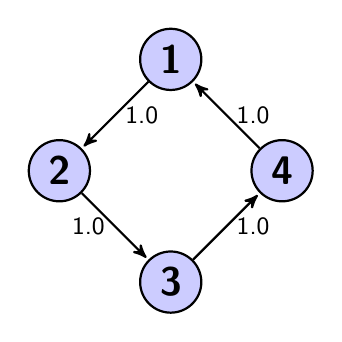
\begin{tikzpicture}[->,>=stealth',shorten >=1pt,auto,node distance=2cm,
  thick,main node/.style={circle,fill=blue!20,draw,font=\sffamily\Large\bfseries}]

  \node[main node] (1) {1};
  \node[main node] (2) [below left of=1] {2};
  \node[main node] (3) [below right of=2] {3};
  \node[main node] (4) [below right of=1] {4};

  \path[every node/.style={font=\sffamily\small}]
    (1) edge node [right] {1.0} (2)
    
    (2) edge node[left] {1.0} (3)
    
    (3) edge node[right] {1.0} (4)
    
    (4) edge node[right] {1.0} (1);
\end{tikzpicture}\end{center}


From the graph we can see any two nodes can communicate and thus (b) is irreducible.

(c)  

\begin{center}
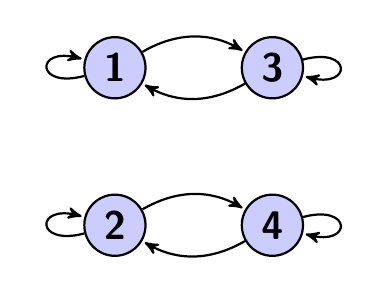
\begin{tikzpicture}[->,>=stealth',shorten >=1pt,auto,node distance=2cm,
  thick,main node/.style={circle,fill=blue!20,draw,font=\sffamily\Large\bfseries}]

  \node[main node] (1) {1};
  \node[main node] (3) [right of=1] {3};
  \node[main node] (2) [below   of=1] {2};
  \node[main node] (4) [ right of=2] {4};

  \path[every node/.style={font=\sffamily\small}]
    (1) edge [loop left] node[left] {} (1)
    	edge [bend left] node [left] {} (3) 
    	
    (2) edge [loop left] node[left] {} (2)
    	edge [bend left] node[right] {} (4)
    	
    (3) edge [bend left] node[right] {} (1)
    	edge [loop right] node[right] {} (3)
    	
    (4) edge [bend left] node[right] {} (2)
    	edge [loop right] node[right] {} (4);
\end{tikzpicture}
\end{center}


From state class, easily we can see four states are categorized into two
communicating classes $\set{\snum{1},\snum{3}}$ and 
 $\set{\snum{2},\snum{4}}$. So (c) is reducible.\\

(d) \par


\begin{center}
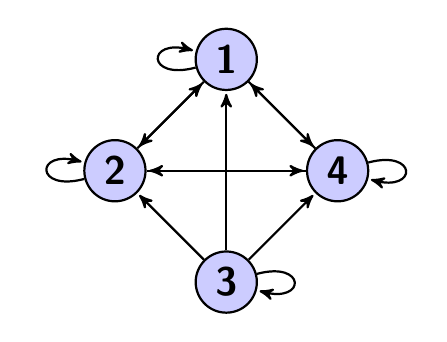
\begin{tikzpicture}[->,>=stealth',shorten >=1pt,auto,node distance=2cm,
  thick,main node/.style={circle,fill=blue!20,draw,font=\sffamily\Large\bfseries}]

  \node[main node] (1) {1};
  \node[main node] (2) [below left of=1] {2};
  \node[main node] (3) [below right of=2] {3};
  \node[main node] (4) [below right of=1] {4};
  
  \path[every node/.style={font=\sffamily\small}]
    (1) edge [loop left] node[left] {} (1)
    	edge node [left] {} (2)
    	edge node [left] {} (4) 
    	
    (2) edge node [left] {} (1)
    	edge [loop left] node [left] {} (2)
    	edge node [left] {} (4)
    	
    (3) edge node [left] {} (1)
    	edge node [left] {} (2)
    	edge [loop right] node [left] {} (3)
    	edge node [left] {} (4)
    	
    (4) edge node [left] {} (1)
    	edge node [left] {} (2)
    	edge [loop right] node [left] {} (4);
\end{tikzpicture}
\end{center}

The state \snum{3} is not accessible from  any other state, and thus (d) is reducible.\\
 



\Exercise[origin={p55, 2.20}]
 Classify the irreducible DTMCs with the transition matrices given below as
periodic or aperiodic:\\

\Answer
(a) From 2.19, we have (a) is aperiodic.\par
(b) $d = 4$.\par
(c) $d = 2.$\par
(d) $d = 3.$\par
PS: try yourself to draw graph like before, and you can easily see the period from the graph.
 

 
\Exercise[origin={p56, 2.21}]
 Compute a normalized solution to the balance equations for the DTMC in
Computational Problem 2.20(a). When possible, compute:
\begin{itemize}
\item[1.]the limiting distribution;
\item[2.]the stationary distribution;
\item[3.]the occupancy distribution.
\end{itemize}
\Answer
\par

(a) is a finite-state irreducible aperiodic DTMC, which has unique limiting distribution, stationary distribution and occupancy distribution, denoted as $\pi, \mu,\nu$.
Solve the balance equation
\[
\pi=\pi P
\]
\[
\pi=\mu=\nu= \begin{bmatrix}
	0.1703&
    0.2297& 
    0.2687& 
    0.3313
\end{bmatrix}.
\]
\vspace{1\baselineskip}





\Exercise[origin={p57, 2.28}]
 Consider the weather model of Conceptual Problem 2.13. Compute the long-run fraction of days that are sunny.\\

\Answer\par
Compute the occupancy distribution, denoted as $\nu$.
\[
\nu=\nu P.
\]
Its solution is 
\[
\nu=\begin{bmatrix}
0.3736 & 0.2126 & 0.2011 & 0.2126
\end{bmatrix}
\]
The long-run fraction of days that are sunny is $37.36\%$.\\



\Exercise[difficulty=2]


   We consider  the annual  movement of a stock market as a three-state DTMC 
with the transition diagram as shown in next page.
Suppose that in the year of ``Bull market" , ``Stagnant market"
and ``Bear market",  the return rates  are $15\%$, $0\%$
and $-12\%$ respectively.
Suppose that the investment in money market is no risk at all
with compound annualised interest  rate $5\%$.
As a long-time value investor,  you prefer to investing 
in stock market or money market ? 
\begin{center}
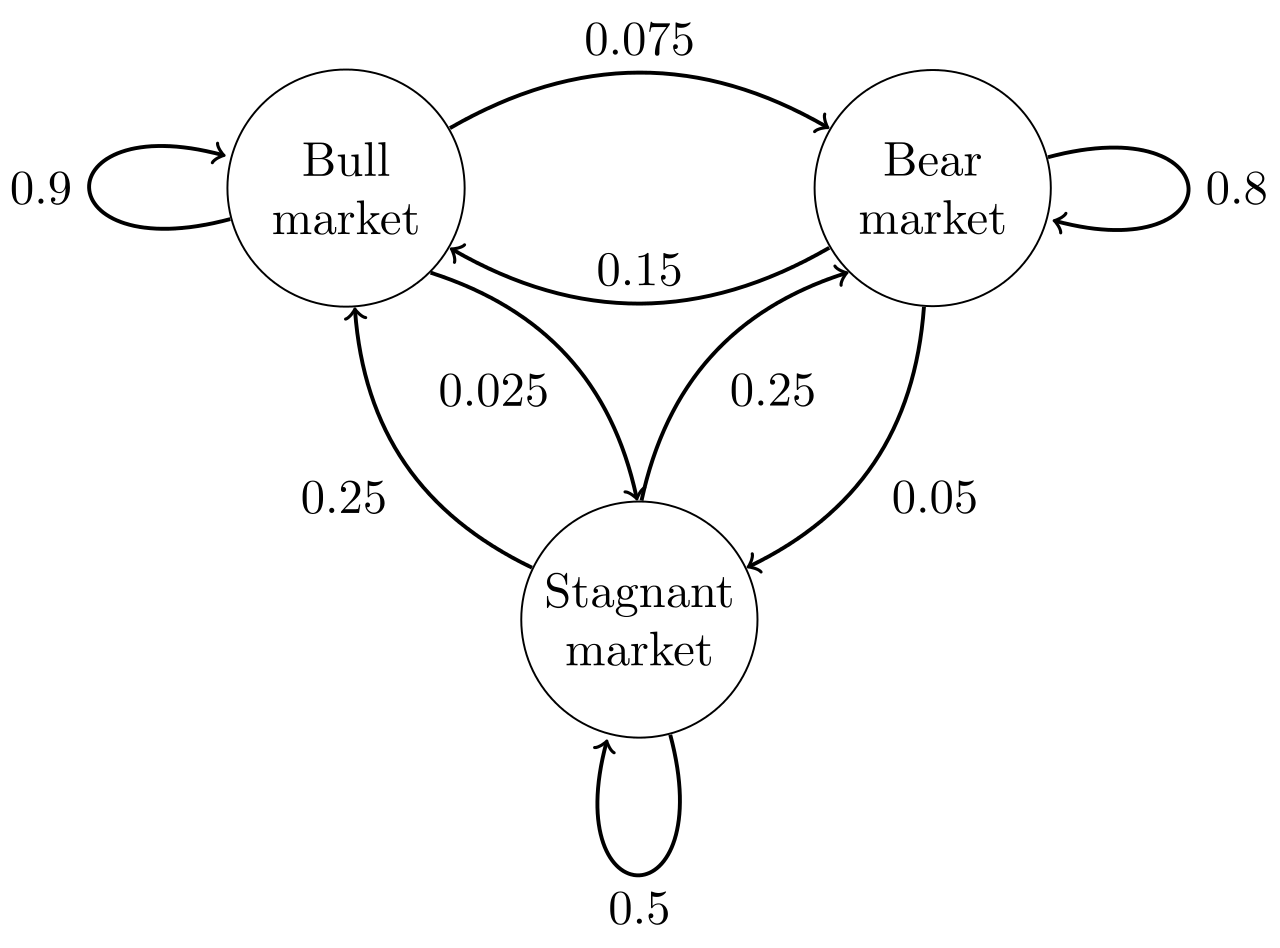
\includegraphics[width=0.6\textwidth]{../StockMarket.png}
\end{center}


\Answer 
Denote ``Bull market", ``Stagnant market", ``Bear Market" by state 1, 2 and 3 correspondingly. 
The Markov chain $X_n$ has the following 
transition probability matrix  $$P = \begin{bmatrix}
0.9 & 0.025 & 0.075 \\
0.25 & 0.5 & 0.25 \\
0.15 & 0.05 & 0.8 
\end{bmatrix}.$$
This DTMC is irreducible and aperiodic and thus has a unique occupancy distribution.
We can find this distribution $\nu = \begin{bmatrix}
0.6250 & 0.0625 & 0.3125
\end{bmatrix}$ by solving the balance equation(see MATLAB code bellow ).


 The return rate is   $r(x) = \begin{bmatrix}
0.15, & 0,  & -0.12
\end{bmatrix}$.
Suppose that initially one unit dollar is invested in this stock market.
Then at the end of the year $n$, the amount of the asset price $s_n$ is 
$s_n = \Pi_{i=1}^n(1+r(X_i))$. Then the annualised return rate is 
$ R_n= (s_n)^{1/n}-1$. We want to compare $\lim_n R_n$ with the money market rate $r_{mm}=5\%$.
After  taking $\log$, 
we need compare $ \lim_n \log (s_n^{1/n})$ with $\log(1+r_{mm})=0.04879$.
 
 Since 
 $ \lim_n \log (s_n^{1/n})= \lim \frac{1}{n} \sum_{i=1}^n \log (1+r(X_i))$,
the cost function is then $c(x):=\log (1+r(x))= [ 0.13976       ,     0,     -0.12783]$.
 In the long run $\lim_n \log (s_n^{1/n}) = (c,\pi) = 0.047403 < 0.04879$. 
 So investigating in money market is preferred.
{\bf Remark:} (1) Here we used the strong ergodicity;
(2) This idealized model is not for any real investment advice;
the variance is not considered here.
\vspace{1\baselineskip}
\begin{lstlisting}
EDU>> P = [0.9  0.025  0.075;
0.25  0.5  0.25;
0.15 0.05 0.8]

P =

    0.9000    0.0250    0.0750
    0.2500    0.5000    0.2500
    0.1500    0.0500    0.8000

EDU>> [V,D] = eigs(P')

V =

    0.8909    0.7366    0.2757
    0.0891   -0.0632   -0.8034
    0.4454   -0.6734    0.5277


D =

    1.0000         0         0
         0    0.7414         0
         0         0    0.4586

EDU>> Pi = V(:,1)/sum(V(:,1))

Pi =

    0.6250
    0.0625
    0.3125

\end{lstlisting}



\end{ExerciseList}




\newpage
\section*{Chapter 2 (part iv)}
\setcounter{Exercise}{0}

\begin{ExerciseList}
\Exercise
For the two-state DTMC with $ {S}=\set{1,2}$ and 
 $\Pm = \begin{bmatrix} 1- a & a \\ b & 1-b \end{bmatrix}$ where 
$a,b\in [0,1]$. 
Let $T_j(i)$ be the first passage time of reaching the state $j$ if $X_0=i$.
$h_j(i)=\e[T_j(i)|X_0=i]$.
(i): 
Calculate $h_1(1)$, $h_2(2)$ %=0
 and $h_2(1)$ and $h_1(2)$. %=1/a, 1/b.
 (ii): What is the distribution of $T_2(1)$? 
 Calculate its expectation by this distribution.
(iii):  Let $T^\rt_j(i)$ be the first return time and $h^\rt_j(i)$ is its expectation.
 Show that if $b>0$, then $h^\rt_1(1)=1+\frac{a}{b}$, $h^\rt_1(2)=\frac{1}{b}$.
 What is the distribution of $T^\rt_1(1)$?
What is the distribution of    $T^\rt_2(1)$?
What is the return probability $\rho_{11}=\p(T^\rt_1(1)<\infty \vert X_0=1)$?
When do we have $\rho_{11}=1$, i.e, the state $1$ is recurrent ?
 \Answer
\par
\begin{enumerate}
\item[(i)]: 
$h_1(1)=h_2(2)=0$ since $T_i(i)=0$ almost surely.
Since $h_2(1)= p_{11}(1+h_2(1)) + p_{12}(1+h_2(2))=(1-a)(1+h_2(1)) + a $,
then $h_2(1)=1/a$ if $a>0$; otherwise $h_2(1)=\infty$.
For the same reason  $h_1(2)=1/b$ if $b>0$;   $h_1(2)=\infty$ if $b=0$. 
\item[(ii)]: It is clear that $T_j(i) \geq 1$ for any $i\neq j$.
$\p(T_2(1)=1)=\p( X_1 =2 \vert X_0=1 )=p_{12}=a$.
For any $k\geq 2$,   
\[
\begin{split}
\p(T_2(1)=k)&=\p( X_{k}=2, X_{k-1} \neq 2, \ldots, X_1\neq 2 \vert X_0=1 )
\\
&=\p( X_{k}=2, X_{k-1} =1, \ldots, X_1=1 \vert X_0=1 )
\\
&=p_{11}p_{11}\ldots p_{11} \times p_{12}=(1-a)^{k-1}\times a
\end{split}
\]
So,
$\p(T_2(1)<\infty)=  \sum _{k=1}^\infty  (1-a)^{k-1} a =a  \cdot (1/a)=1 $ if $a>0$.
The expectation is 
\[\begin{split} h_2(1)&=\e(T_2(1)) = \sum _{k=1}^\infty  k(1-a)^{k-1} \times a  \\
&= a \times \frac{d}{da}(-\sum _{k=1}^\infty  (1-a)^{k})\\
&=a \times ( 1/a^2)=1/a
\end{split} \]
if $a>0$. This direct calculation matches our previous result
from the ``one-more-step'' analysis.

\item[(iii)]:  
$T^\rt_j(i)=T_j(i)$ if $i\neq j$.
So $h^\rt_1(2)=h_1(2)=\frac{1}{b}$
and $T^\rt_1(2)$ has the same distribution of $T_2(1)$.

Now we work on $T^\rt_1(1)=\inf\set{n\geq 1:  X_n =1\vert X_0=1}$,
which takes value in $1,2,\ldots$. 
$\p(T^\rt_1(1)=1)=\p(X_1=1 \vert X_0=1)=1-a$.
For $k\geq 2$, then 
$\p(T^\rt_1(1)=k)=\p(X_k=1, X_{k-1}=2,\ldots, X_1=2 \vert X_0=1)=
p_{12}p_{22}p_{22}\ldots p_{22}p_{21}=(1-b)^{k-2}ab$.
Then
\[\rho_{11}= \sum_{k=1}^\infty\p(T^\rt_1(1)=k)  =1-a + \sum_{k=2}^\infty  (1-b)^{k-2} ab=
1-a+ab /b =1 \]
if $b>0$.

If $b=0$, then $$\rho_{11}=   \p(T^\rt_1(1)=1) + 0 =1-a$$
and $$\p(T^\rt_1(1)=\infty)=1-\rho_{11}=a.$$

So, the state $1$ is recurrent (i.e. $\rho_{11}=1$) if and only if  $b>0 $ 
or $a=b=0$.

Now we calculate   $h^\rt_1(1)$.
By the ``one-more-step'' analysis
$h^\rt_1(1) = p_{11} \times 1 \xout{( 1+ h^\rt_1(1))} + p_{12} (1+h^\rt_1(2))
= (1-a) \times {\color{blue}{1}} + a (1+h_1(2))=1+a/b$
since $h^\rt_1(2)=h_1(2)=b$.
On the other hand, we can compute $h^\rt_2(1)$ as follows:
\[
\begin{split}
h^\rt_1(1) &= \sum_{k=1}^\infty k \times \p(T^\rt_1(1)=k)
\\
&=(1-a) + \sum_{k=2}^\infty  k(1-b)^{k-2} ab
\\
&=(1-a) + \sum_{k=1}^\infty  (k+1)(1-b)^{k-1} ab
\\
&=(1-a) + a + \sum_{k=1}^\infty  k(1-b)^{k-1} a\times b
\\
&=1  + (1/a) \times b = 1+a/b,
\end{split}
\]
\end{enumerate}
if $b>0$.
So, the state $1$ is also positive recurrent if $b>0$.
If $b=0$, then the above shows that $h^{\rt}_1(1)=1\times (1-a) +a\times \infty $, the state $1$
is  positive recurrent if and only if $a=0$.
So,
 the state $1$ is positive recurrent (i.e. $h^\rt_{1}(1)<\infty$) if and only if  $b>0 $ 
or $a=b=0$.



\Exercise
For Gambler's Ruin Problem (Example 2.33, page 43), what is the expected dollars of gambler A when the game stops?\\

\Answer
 Set A $ = \{0,N\}$, $S  = \{0,1,\dots, N\}$.\par
\[\begin{split}
\mathbb{E}[X_{T_A} \mid X_0 = i] %& = \sum_{j\in S} j \mathbb{P}[X_{T_A} = j \mid X_0 = i] \\
& = 0\times \mathbb{P}[X_{T_A} = 0 \mid X_0 = i] + N\times \mathbb{P}[X_{T_A} = N \mid X_0 = i] \\
& = N\times \mathbb{P}[X_{T_A} = N \mid X_0 = i] \\
& = N g_{N}(i) 
\end{split}\]

If $i = 0$, $g_{N}(i) = \mathbb{P}[X_{T_A} = N \mid X_0 = i] = 0$.\par
If $i = N$, $g_{N}(i) = \mathbb{P}[X_{T_A} = N \mid X_0 = i] = 1$.\par
For $i\in \{1,2,...,N-1\}$,
\[\begin{split}
g_{N}(i) & = \sum_{j\in S} \mathbb{P}[X_{T_A} = N \mid X_0 = j]P_{ij} \\
& = \sum_{j\in S} g_{N}(j)P_{i,j}\\
& = g_{N}(i+1) P_{i,i+1} + g_{N}(i-1) P_{i,i-1} \\
& = g_{N}(i+1) p + g_{N}(i-1)(1-p)
\end{split}\]

Denote $g_{N}(i) $ by $g_{i}$ for simplicity. $g_{0} = 0 
\text{ \& } g_{N} = 1$. $g_i = g_{i+1}p+g_{i-1}(1-p)$.
\[ p(g_{i+1} -g_{i}) = (1-p)(g_i - g_{i-1}) \Rightarrow g_{i+1} - g_{i} = \frac{1-p}{p} (g_i - g_{i-1})\] Denote $\frac{1-p}{p}$ by $\alpha$. Hence, 
\[g_{i+1} - g_{i} = \alpha (g_i - g_{i-1}) \text{ }\forall i \in \{1,2,...,N-1\} \]
Assume $g_1 = x$, so $g_1 - g_0 = x$. $g_{i+1} - g_{i} = \alpha^{i} (g_1-g_0) = \alpha^{i} x \text{, } \forall i \in \{1,2,...,N-1\}$. $\because 1 = g_{N} = g_0 + \sum_{i=0}^{N-1} (g_{i+1}-g_{i}) = \sum_{i=0}^{N-1} (g_{i+1}-g_{i}) = \sum_{i=0}^{N-1} \alpha^{i} x \Rightarrow \frac{1-\alpha^N}{1-\alpha} x = 1$, so $x =  \frac{1-\alpha}{1-\alpha^N}$. $g_{i+1} = g_{0} + \sum_{j=0}^{i} (g_{j+1}-g_{j}) = \sum_{j=0}^{i} \alpha^{j}x = \frac{1-\alpha^{i+1}}{1-\alpha}\frac{1-\alpha}{1-\alpha^N} = \frac{1-\alpha^{i+1}}{1-\alpha^{N}}$. Hence,
\[\begin{split}
g_{N}(i) = g_{i} = & \frac{1-\alpha^i}{1-\alpha^N}\text{ }\forall j \in S \\
\mathbb{E}[X_{T_A} \mid X_0 = i] & = N\frac{1-\alpha^i}{1-\alpha^N} \text{ where } \alpha = \frac{1-p}{p}
\end{split}
\]

The special case that $p=1/2$, i.e., $\alpha=1$, then
\[
\mathbb{E}[X_{T_A} \mid X_0 = i]  = N\frac{i}{ N} = i =X_0
\]
This means if $p=1/2$, the game is quite``fair"
($\set{X_n}$ is martingale):  on average,
what the player A has when the game stops is equal to what he initially brings in.
He can not  make guaranteed profit from the game. 

\Exercise

Consider the symmetric random walk on $S=\set{1,\ldots,N}$ with periodic boundary on two ends
$1$ and $N$. Find the mean first passage time to $N$ if starting from $1$, i.e.,
 $\e( T_{\set{N}}  | X_0=1)$.
 Find the expected return time $h_1^\rt(1)=\e T^\rt_1(1)$.


\Answer
Set $h_i =\e( T_{\set{N}}  | X_0=i)$ for simplicity.
Then $h_N=0$ and
\[  h_{i}= (1+h_{i+1})/2 + (1+h_{i-1})/2  ,  ~~~i =1,2,\ldots, N-1  \]
where $h_{0}=h_{N}=0$ by periodic boundary condition
(state $0$ is identical to state $N$).
So $2h_{i}= 2+ h_{i+1} + h_{i-1}$ and 
$h_{i+1}-h_{i}=h_i-h_{i-1}-2 =(h_{i-1}-h_{i-2}-2)-2
=\ldots=h_1-h_0 - 2*i=h_1-2i$, then
taking sum over $i=0,1,\ldots,k(\leq N-1)$,
we have $h_{k+1}-h_0= (k+1) h_1 - 2\sum_{i=0}^{k}i=
(k+1) h_1 - (k+1)k$.
So, $h_{k+1}=(k+1) (h_1-k)$.
In particular $k=N-1$ gives  $0=h_N=N(h_1-(N-1))$. So,
\[h_1 =  N-1\]
and $h_i = i (N-i)$ for $1\leq i\leq N$.

{\bf Remark:}  $f''(x)=-2$ with boundary $f(0)=f(1)=0$ has the solution  $f(x)=x(1-x).$

{\bf Remark: } To find  $h_j(i) =\e( T_{\set{j}}  | X_0=i)$ for any $i,j$,
we first note the symmetry gives that $h_{j}(i)=h_{i}(j)$.
So we assume that $j>i$ in calculating $h_j(i)$.
By symmetry again, we relabel the state  space by the order 
$j\to  {N}$, $j-1\to  {N-1},\ldots$,
$i\to  i':= i+ (N-j)$.
Then $h_{j}(i)=h_N(i')=i'(N-i') = (j-i) ( N - (j-i))
=\abs{j-i} \times (N  - \abs{j-i})$ in general.
which is the product of two arc length steps 
connecting  two states on a circle.

The return time 
$h^\rt_1(1)
= \left( \sum_{k\neq 1} h_1(k) p_{1k} \right) +1=
h_1(2)/2 + h_1(0)/2+1
=(N-1)/2+(N-1)/2+1=N$.

\Exercise[origin={p57 2.42}] Compute the expected time to go from state 1 to 4 in the DTMCs of Computational Problems 2.20(a) and (c).\\

\Answer:
Denote $\mathbb{E}[T_A \mid X_0 = i]$ by $h_{A}(i)$ where $A = \{4\}$. For $i \notin A$, $h_{A}(i) = 1 + \sum_{j\in S} h_{A}(j)P_{i,j}$. $h_{A}(4) = 0$.\par
Denote $\begin{bmatrix}
h_A(1)\\h_A(2)\\h_A(3)
\end{bmatrix}$ by $h$, $\begin{bmatrix}
P_{11} &P_{12} &P_{13} \\
P_{21}& P_{22} &P_{23} \\
P_{31} &P_{32}& P_{33} \\
\end{bmatrix}$ by $P$, and $\begin{bmatrix}
1 \\ 1 \\ 1
\end{bmatrix}$ by $b$

\[h = Ph+b\]
\[(P-I)h = -b\]

For (a)
\[
h_1=1+0.1h_1+0.3h_2+0.2h_3
\]
\[
h_2=1+0.1h_1+0.3h_2+0.4h_3
\]
\[
h_3=1+0.3h_1+0.1h_2+0.1h_3
\]
$[h_1, h_2, h_3] \approx \begin{bmatrix}
	2.6887 &
    3.1604 &
    2.3585
\end{bmatrix}$\\

For (c), 
\[
h_1=1+0.2h_2+0.3h_4
\]
\[
m_2=1+m_1
\]
\[
m_3=1+m_1
\]
The result is $[h_1, h_2, h_3] = \begin{bmatrix}
	3 &
    4 &
    4
\end{bmatrix}$

Matlab code is attached as your reference.
\begin{lstlisting}
EDU>> P = [0.1, 0.3, 0.2; 0.1, 0.3, 0.4; 0.3, 0.1, 0.1]

P =

    0.1000    0.3000    0.2000
    0.1000    0.3000    0.4000
    0.3000    0.1000    0.1000

EDU>> b = ones(3,1);
EDU>> h = (P-eye(3,3))\(-b)

h =

    2.6887
    3.1604
    2.3585

EDU>> P = [0, 0.2, 0.3; 1, 0, 0; 1, 0, 0]

P =

         0    0.2000    0.3000
    1.0000         0         0
    1.0000         0         0

EDU>> h = (P-eye(3,3))\(-b)

h =

     3
     4
     4
\end{lstlisting}
\vspace{2\baselineskip}


 

\Exercise[origin={p57, 2.43}] Compute the expected time to go from state 1 to 4 in the DTMCs of Computational Problems 2.20(b) and (d).\\
\Answer
\par
(b) $\begin{bmatrix}
h_1 & h_2 & h_3
\end{bmatrix} = \begin{bmatrix}
3 & 2 & 1
\end{bmatrix}$

(d) $\begin{bmatrix}
h_1 & h_2 & h_3
\end{bmatrix} = \begin{bmatrix}
3 & 4 & 5
\end{bmatrix}$ 
 



\Exercise[name=\optional, difficulty=5] The Department of Security  has  three floors, 0th(ground), 1st  and 2nd floor.
Each floor has three rooms: Room $A$, $B$ and $C$ from left to right.
Let $A_i$ be the room $A$ at Floor $i$ , $i=0,1,2$. $B_i$ and $C_i$ are defined likewise.
There is a door between two  neighbouring rooms at the same level.
It is also possible to break windows to climb upstair or downstair vertically into the room on the neighbouring floor. See figure for illustration.

 \begin{center}
\begin{tabular}{|c|c|c|}
\hline
A2 & B2 & C2 \\
\hline
A1 & B1 & C1 \\
\hline
A0 & B0 & C0 \\
\hline
\end{tabular}
\end{center}

The only exit of this building is located in Room $B_0$.
At initial time,  there is a spy at Room $C_2$,   unfortunately  triggering  the security alarm 
and without knowing which room is exit unless inside this room,  he starts to run in panic randomly in this building. At each step,  the spy, with equal probability, moves to one of  the rooms that he can access
through  doors (taking $2$ seconds)  or by  breaking windows (taking $15$ seconds). On average, how much time does the spy need to escape this building? \\

\Answer

Denote A0, B0, C0, A1, B1, C1, A2, B2, C2 sequentially by state 1 to 9. $S = \{1, 2, \dots, 9\}$. The transition matrix is
\[P = \begin{bmatrix}
0 & \frac{1}{2} & 0 & \frac{1}{2} & 0 & 0 & 0 & 0 & 0 \\
\frac{1}{3} & 0 & \frac{1}{3} & 0 & \frac{1}{3} & 0 & 0 & 0 & 0 \\
0 & \frac{1}{2} & 0 & 0 & 0 & \frac{1}{2} & 0 & 0 & 0 \\
\frac{1}{3} & 0 & 0 & 0 & \frac{1}{3} & 0 & \frac{1}{3} & 0 & 0 \\
0 & \frac{1}{4} & 0 & \frac{1}{4} & 0 & \frac{1}{4} & 0 & \frac{1}{4} & 0 \\
0 & 0 & \frac{1}{3} & 0 & \frac{1}{3} & 0 & 0 & 0 & \frac{1}{3}\\
0 & 0 & 0 & \frac{1}{2} & 0 & 0 & 0 & \frac{1}{2} & 0 \\
0 & 0 & 0 & 0 & \frac{1}{3} & 0 & \frac{1}{3} & 0 & \frac{1}{3} \\
0 & 0 & 0 & 0 & 0 & \frac{1}{2} & 0 & \frac{1}{2} & 0\\
\end{bmatrix} \]

The cost matrix \[C = \begin{bmatrix}
0 & 2 & 0 & 15 & 0 & 0 & 0 & 0 & 0 \\
2 & 0 & 2 & 0 & 15 & 0 & 0 & 0 & 0 \\
0 & 2 & 0 & 0 & 0 & 15 & 0 & 0 & 0 \\
15 & 0 & 0 & 0 & 2 & 0 & 15 & 0 & 0 \\
0 & 15 & 0 & 2 & 0 & 2 & 0 & 15 & 0 \\
0 & 0 & 15 & 0 & 2 & 0 & 0 & 0 & 15 \\
0 & 0 & 0 & 15 & 0 & 0 & 0 & 2 & 0 \\
0 & 0 & 0 & 0 & 15 & 0 & 2 & 0 & 2 \\
0 & 0 & 0 & 0 & 0 & 15 & 0 & 2 & 0\\
\end{bmatrix}\]
where $C_{i,j}$ means the time cost of this spy if he wants to run or climb from state $i$ to $j$.\\

Denote $h(i)$ as $\mathbb{E} [T_A | X_0 = i]$, where $A = \{2\}$, and $T_A$ means the hitting time into set A. Thus $h(2) = 0$. For $i\in (S\setminus A)$, $h(i) = \sum_{j\in S} P_{ij}(C_{ij} + h(j))$.\\

Denote $\tilde{P}$ as a modification of matrix $P$ with elements in row 2 as 0. Then, \[h(i) = \sum_{j\in S} \tilde{P}_{ij}(C_{ij} + h(j))\] is true for {\it all} $i\in S$. Denote $h$ as a column vector with row i as $h(i)$.
and denote $b$ as a column vector with row i as $b(i) = \sum_{j\in S} \tilde{P}_{i,j}C_{i,j}$. Hence, 
\[h = \tilde{P}h + b\]

With the assistance of Matlab,  
$$h = [53.1667 ,
         0  ,
   53.1667,  
   89.3333 ,
   78.6667 ,
   89.3333 ,
  104.1667 ,
  102.0000 ,
  104.1667
]^T$$
Hence the result is $h(9) = 104.1667$.
\newpage
Matlab code is attached as reference:
\begin{lstlisting}
% input matrix
P = [0, 1/2, 0, 1/2, 0, 0, 0, 0, 0;
    1/3, 0, 1/3, 0, 1/3, 0, 0, 0, 0;
    0, 1/2, 0, 0, 0, 1/2, 0, 0, 0;
    1/3, 0, 0, 0, 1/3, 0, 1/3, 0, 0;
    0, 1/4, 0, 1/4, 0, 1/4, 0, 1/4, 0;
    0, 0, 1/3, 0, 1/3, 0, 0, 0, 1/3;
    0, 0, 0, 1/2, 0, 0, 0, 1/2, 0;
    0, 0, 0, 0, 1/3, 0, 1/3, 0, 1/3;
    0, 0, 0, 0, 0, 1/2, 0, 1/2, 0];
C = [0, 2, 0, 15, 0, 0, 0, 0, 0;
    2, 0, 2, 0, 15, 0, 0, 0, 0;
    0, 2, 0, 0, 0, 15, 0, 0, 0;
    15, 0, 0, 0, 2, 0, 15, 0, 0;
    0, 15, 0, 2, 0, 2, 0, 15, 0;
    0, 0, 15, 0, 2, 0, 0, 0, 15;
    0, 0, 0, 15, 0, 0, 0, 2, 0;
    0, 0, 0, 0, 15, 0, 2, 0, 2;
    0, 0, 0, 0, 0, 15, 0, 2, 0];
% now P become \tilde{P} as is in the analysis part
P(2,:) = zeros(1,9); 
b  = sum(P.*C,2);
% result
h = (P-eye(9,9))\(-b);
\end{lstlisting}

 
\end{ExerciseList}




\newpage
\section*{Chapter 3 }
\setcounter{Exercise}{0}

\begin{ExerciseList}

\Exercise(Minimum of Exponentials) 
$X = \min\{X_1,X_2,...,X_k\}$,  where $\{X_i\}$ are independent $\Exp(\lambda_i)$ random variables, is an $\Exp(\lambda)$ random variable, where 
\[\lambda = \sum_{i=1}^{k} \lambda_i \]


\Answer
If $X_i > x$ for all $1\le i\le k$, then $X > x$ and vice versa. Using this and the independence of $X_i$, $1\le i \le k$, we get
\[\begin{split}
\p(X>x) & =  \p(\min\{X_1,X_2,...,X_k\} > x) \\
& = \p(X_1>x,X_2>x,...,X_k>x) \\
& = \p(X_1>x) \p(X_2>x)\dots \p(X_k>x) \\
& = e^{-\lambda_1 x}e^{-\lambda_2 x}\dots e^{-\lambda_k x} \\
& = e^{-\lambda x}
\end{split}\]
which shows $X\sim \Exp(\lambda)$. 





\Exercise (Sums of Poisson) Suppose $\{X_i, i = 1, 2, \dots, n\}$ are independent random variables with $X_i \sim \Poi(\lambda_i)$, $1\le i \le n$. Let
\[Z_n = X_1+X_2+\dots + X_n\]
Then $Z_n$ is a $\Poi(\lambda)$ random variable, where 
$\lambda = \sum_{i=1}^{n}\lambda_i$.


\Answer
We shall  first show the result for $n=2$,
then the general result then follows by induction. 
For $k=2$, using equation \[p_Z(z) = \sum_{x_1}p_{X_1}(x_1)p_{X_2}(z-x_1) = \sum_{x_2}p_{X_1}(z-x_2)p_{X_2}(x_2)\] we get
\[\begin{split}
p_Z(k) & = \sum_{k_2 = 0}^{k} e^{-\lambda_1}\frac{\lambda_1^{k-k_2}}{(k-k_2)!}e^{-\lambda_2}\frac{\lambda_2^{k_2}}{k_2 !} \\
& = e^{-\lambda_1-\lambda_2} \frac{1}{k^2}\sum_{k_2=0}^{k}\frac{k!}{(k-k_2)!k_2 !}\lambda_1^{k-k_2}\lambda_2^{k_2} \\
& = e^{-\lambda_1-\lambda_2} \frac{(\lambda_1+\lambda_2)^k}{k!}
\end{split}\]

Thus $Z$ follows $\Poi(\lambda_1+\lambda_2)$. This completes the proof for $n=2$.\\
 
 Now assume $Z_n \sim \Poi(\sum_{i=1}^n\lambda_i)$, we need show
 $Z_{n+1}=Z_n + X_{n+1}  \sim \Poi(\sum_{i=1}^n\lambda_i + \lambda_{n+1})$,
 which is the direct result when the above $n=2$ case is applied
 for two independent  Poisson r.v.s $Z_n$ and $X_{n+1}$.



\medskip

\textbf{Alternative proof}:
There is a one-to-one relation between the   generation function
and the distribution density. 
 Consider the generating function 
$g_X(s) := \e(e^{s X}),~ s>0$   for any random variable $X$.
If   $X$ is a Poisson r.v. $\Poi(\lambda)$, then 
\[ g_X(s)= \sum_{k\geq 0} e^{sk}  e^{-\lambda} \frac{\lambda^k}{k\!}
= \sum_{k\geq 0}   e^{-\lambda} \frac{(e^s \lambda)^k}{k\!}=e^{\lambda (e^s-1)}.\]  The reverse is also true:
if $g_X(s)=e^{\lambda (e^s-1) }$, then $X\sim \Poi(\lambda)$.
 
 
 
Now we compute the generation function for the sum of independent Poisson r.v.s $\{X_i\}$.
\[g_{Z_n}(s)=\e(e^{-s X_1-\ldots - s X_n}) = \Pi_{i=1}^n (\e e^{-sX_i}) =
\Pi_{i=1}^ne^{\lambda_i (e^s-1)}
=e^{\sum_{i=1}^n\lambda_i (e^s-1)}
\]
which means $Z_n\sim \Poi(\sum_{i=1}^n \lambda_i)$.


\Exercise [origin={3.9, p79}] 
  Let $X$ be a $\Poi(\lambda)$ random variable. Show that
$$\e[X(X-1)(X-2)\dots(X-k+1)] = \lambda^k, \hspace{0.4cm} k\ge 1$$
 
\Answer: 
From definition of expectation, we have
\[\begin{split}
&\e[X(X-1)(X-2)\dots(X-k+1)] = \sum_{i=0}^{\infty} i(i-1)(i-2)\dots(i-k+1) \p(X=i) \\
&=\sum_{i=k}^{\infty} i(i-1)(i-2)\dots(i-k+1) \p(X=i)
= \sum_{i=k}^{\infty} \frac{i!}{(i-k)!} e^{-\lambda}\frac{\lambda^i}{i!} \\
&= \lambda^k \sum_{i'=0}^{\infty} e^{-\lambda}\frac{\lambda^{i'}}{i'!}
= \lambda^k
\end{split}\]




\Exercise [origin={3.10, p79}] 
  Let $X_1\sim \Poi(\lambda_1)$ and $X_2 \sim \Poi(\lambda_2)$ be two independent random variables. Show that, given $X_1+X_2 = k$,
  \[ X_i\sim\Bin(k,\frac{\lambda_i}{\lambda_1+\lambda_2}), i = 1,2.\]\\
\Answer

When $i=1$, $\p(X_1+X_2=k) = e^{-(\la_1+\la_2)} \frac{(\la_1+\la_2)^k}{k!}$
since $X_1+X_2\sim \Poi(\la_1+\la_2)$. For any $j\leq k$,
\[\begin{split}
&\p(X_1=j|X_1+X_2=k) \\
= & \frac{\p(X_1=j, X_2=k-j)}{\p(X_1+X_2=j)} \\
= & \frac{\p(X_1=j) \p( X_2=k-j)}{\p(X_1+X_2=j)} \\
= &\frac{e^{-\la_1}\frac{\la_1^j}{j!}e^{-\la_2}\frac{\la_2^{k-j}}{(k-j)!} }{e^{-(\la_1+\la_2)}\frac{(\la_1+\la_2)^k}{k!}}\\
= & {k \choose j} p^{j}(1-p)^{k-j} 
\end{split}\]
where  $p=\frac{\la_1}{\la_1+\la_2}$.
Thus $X_1\sim \Bin(k,\frac{\lambda_1}{\lambda_1+\lambda_2})$. 
The distribution of $X_2$ can be similarly obtained.\\

\Exercise [origin={3.17, p79}] 
  Let $\{N(t), t\ge 0\}$ be a $\PP(\lambda)$. Let $S_k$ be the time of occurrence of the $k$th event in this Poisson process. Show that, given $N(t)=1$, $S_1$ is uniformly distributed over $[0,t]$.\\

\Answer
Since $\{S_1 \leq x\} =\{N(x)\geq 1\}$ and 
 $N(x)\leq N(t)$ for any $x\leq t$,
 then for any $x\in [0,t]$,
\[\begin{split}
&\cPr{S_1\le x}{ N(t)=1} \\
= &\frac{\p( 1 \leq  N(x) \leq N(t) \ , \ N(t)=1)}{\p(N(t)=1)}\\
= &\frac{\p(  N(x) =1 \ ,\ N(t)=1)}{\p(N(t)=1)}
\\
= & \frac{\p(  N(x) =1 \ ,\ N(t)-N(x)=0)}{\p(N(t)=1)}
\\
=  &\frac{\p(  N(x) =1) \p ( N(t)-N(x)=0)}{\p(N(t)=1)}
\\
=& \frac{e^{-\la x} (\la x) e^{-\la(t-x)}}{e^{-\la t}(\la t)}\\
= & \frac{x}{t}.
\end{split}\]
So $S_1$ is uniformly distributed over $[0,t]$.
  
 
\Exercise [origin={3.19, p80}] 
Let $\{N(t), t\ge 0 \}$ be a $\PP(\lambda)$. Let $s,t\ge 0$. Compute the joint distribution
$$\p(N(s) = i, N(s+t) = j), ~~~0\le i\le j< \infty$$

\Answer
\[\begin{split}
\p(N(s) = i, N(s+t) = j) &= \p(N(s)=i, N(s+t)-N(s)=j-i) \\
&= \p(N(s)=i)\p(N(t)=j-i)\\
&= e^{-\la s} \frac{(\la s)^i}{i!} e^{-\la t}\frac{(\la t)^{j-i}}{(j-i)!}\\
&= e^{-\la(s+t)}\la^j \frac{s^i t^{j-i}}{i!(j-i)!}
\end{split}\]

Remark: the solution in the textbook has  wrong sign.\\

\Exercise [origin={3.20, p80}] 

  Let $\{N(t), t\ge 0 \}$ be a $PP(\lambda)$. Show that 
$$Cov(N(s), N(s+t)) = \lambda s, \hspace{0.4cm}s,t \ge 0$$

\Answer
\[\begin{split}
&Cov(N(s),N(s+t)) \\
&= \e[(N(s)-\la s)(N(s+t)-\la (s+t))]\\
&= \e[N(s)N(s+t)]-\la s \e[N(s+t)]-\la(s+t)\e[N(s)]+\la^2s(s+t)\\
&= \e[N(s)(N(s+t)-N(s))+N(s)^2] - \la^2s(s+t)\\
&= \la s \la t + \la s + (\la s)^2 -\la^2 s(s+t)\\
&= \la s
\end{split}\]

\Exercise [origin={3.25, p80}] 

(3.25 p80) Let $\{C(t), t\ge 0 \}$ be a CPP of Definition 3.6. Compute $Cov(C(t+s),C(s))$ for $s,t\ge 0$.\\

\Answer
The method to compute this is similar to that for exercise 1.3. From exercise 1.3 we know that $\e[C(t)] = \tau \la t$ and $Var(C(t)) = \la t \mu^2$ where $\tau$ is the mean of $C_n$ and $\mu^2$ is the second moment of $C_n$ ($\mu$ is used to avoid duplicate use of $s$).
\[\begin{split}
Cov(C(t+s),C(s)) &= \e[(C(t+s)- \tau\la(t+s))(C(s)-\tau \la s)]\\
&= \e[C(t+s) C(s)] - \tau\la(t+s)\e[C(s)] - \tau\la s\e[C(t+s)]\\
&\hspace{0.3cm}+\tau^2\la^2 s(s+t)\\
&= \e[C(t+s)C(s)] - \tau^2\la^2 s(s+t)\\
&= \e[C(s)^2] + \e[C(s) (C(t+s)-C(s))] - \tau^2\la^2 s(s+t)\\
&= \la s \mu^2  + (\tau\la s)^2 + \tau\la s \times \tau \la t - \tau^2\la^2s(s+t)\\
&= \la s \mu^2 = \la s \e[(C_1)^2]
\end{split}\]

Explanation: $C(t+s)-C(s)$ has the same distribution as $C(t)$ and is independent with $C(s)$ due to the independent and stationery  increment for the comound Poisson process
(because $\{C_n\}$ are iid.)

\textbf{remark}: you can also use the characteristic function given in the lecture note to solve this problem.


\Exercise [origin={3.2, p80}] 
  The lifetimes of two car batteries (brands A and B) are independent exponential random variables with means 12 hours and 10 hours, respectively. What is the probability that the Brand B batter outlasts the Brand A battery?
  
\Answer
$X_A \sim \Exp(\frac{1}{12})$, $X_B \sim \Exp(\frac{1}{10})$, $X_A$ and $X_B$ are independent.
\[\begin{split}
P(X_B > X_A) & = \int_{0}^{\infty} P(X_B > X_A \mid X_A = x) f_A(x) dx  ~~~\mbox{law of total prob.} \\
& = \int_{0}^{\infty} P(X_B > x \mid X_A =x) f_A(x) dx \\
& = \int_{0}^{\infty} P(X_B > x) f_A(x) dx ~~~~\mbox{independent}\\
& = \int_{0}^{\infty} e^{-\lambda_B x} \lambda_A e^{-\lambda_A x} dx\\
& = \frac{\lambda_A}{\lambda_A + \lambda_B} = \frac{\frac{1}{12}}{\frac{1}{12}+\frac{1}{10}} \simeq 45.5\%
\end{split} \]

\Exercise [origin={3.3, p80}] 
Suppose a machine has three independent components with $Exp(.1)$ lifetimes. Compute the expected lifetime of the machine if it needs all three components to function properly.\\

\Answer
$X_i \sim \Exp(.1)$ for $i=1,2,3$.
Let $Z = \min \{X_1,X_2,X_3\}$. Then according to Thm 3.3, $Z \sim \Exp(.3)$, so $\e(Z) = \frac{1}{0.3} \simeq 3.33$.\\
 
\Exercise [origin={3.29, p83}] 
  The number of cars visiting a national park forms a $\PP$ with rate 15 per hour. Each car has $k$ occupants with probability $p_k$ as given below:
$$p_1 = .2, p_2 = .3, p_3 = .3, p_4 = .1, p_5 = .05, p_6 = .05$$
Compute the mean and variance of the number of visitors to the park during a 10-hour window.

\Answer
The number of cars at time $t$ follows a $\PP(15)$.
The number of visitors at the $n$-th car $C_n$ is a random variable taking value between 1 and 6
with the given probability $\{p_k\}$. The total number of visitor at time $t$ is a compound Poisson process
\[C(t)=\sum_{n=1}^{N(t)} C_n.\]

The mean of $C_1$ is $\tau = 2.65$.
The second moment $\e C_1^2$ is $s^2 = 8.75$, thus $\e[\sum_{n=1}^{N(10)} C_n] = \tau \la t = 2.65\times 15\times 10 = 397.5$ and $Var(\sum_{n=1}^{N(10)} C_n) = \la t s^2 = 15\times 10\times 8.75 = 1312.5$.

\Exercise [origin={3.30, p83}] 
Now suppose the national park of Computational Problem 3.29 charges $\$4.00$ per car plus $\$1.00$ per occupant as the entry fee. Compute the mean and variance of the total fee collected during a 10-hour window.

\Answer
The fee collected for the $n$-th car is  $4+ C_n$. So 
The fee collected at time $t$ is 
\[\tilde{C}(t)=\sum_{n=1}^{N(t)} \tilde{C}_n: =\sum_{n=1}^{N(t)} (4+1\times C_n).\]

Now the $\tilde{C}_n=4+C_n$ becomes $i+4$ with probability $p_i$, for $1\le i \le 6$. $\tau = 6.65$, $s^2 = 45.95$. Thus the calculation again shows expectation is $997.5$ and variance is $6892.5$.
 
 \Exercise 
 Let $N$ be a Poisson process with parameter $\lambda$.
Let $U_t$ denote the time of the first observation
{\it after}  time $t$. (In particular, $U_0$ = $S_1$.)
 Calculate the probability density function for $U_t$.
 
\Answer
\[
\p(U_t > s )  =\p ( \text{ no events between } (t, t+s] ~)
= \p  (N(t+s)-N(s)=0  )=e^{-\lambda s }
\]
so $U_t \sim Exp(\lambda)$     (independent of $t$ ! Recall the memoryless property).



 
\Exercise
Let $N(t)$ be the number of arrival customers
and assume $\{N(t)\}$ is  a Poisson process with rate $ \lambda$. $S_n$ is the $n$th jump time.
Let  $t_i = i$ for $i=1,2,3,4$.
\begin{enumerate}
\item  What is the expected number of arrival customers at time $t_4$?
\item  What is the probably that there are no arrivals from $t_1$ to $t_3$?
\item What is the probably that there are two arrivals  from $t_1$ to $t_3$
and one arrives before $t_2$ and the other arrives after $t_2$ ?
\item What is the probably that there are two arrivals  from $t_1$ to $t_4$
and one arrives before $t_3$ and the other arrives after $t_2$ ?
\item $\mathbb{P}(N(t_3) =5|N(t_1) =1)=?$
\item $\mathbb{E}(N(t_2)N(t_1)) = ? $
\item  $\mathbb{E} [N(t_1)N(t_4)(N(t_3) -N(t_2))] = ?$
\item $\e [N(t_2)\mid S_1 > t_1] = ?$
\item $\mathbb{E}[N(t_2) \mid  S_2 >t_1] = ? $
\end{enumerate}


\Answer
\begin{enumerate}
\item $N(t_4) \sim \Poi(\lambda t_4)$, so $\mathbb{E}[N(t_4)] = \lambda t_4 = 4\lambda$.

\item $ \mathbb{P}(N(t_3)-N(t_1) = 0) = \mathbb{P}(N(t_3-t_1)=0) = e^{-\lambda (t_3-t_1)} = e^{-2\lambda}$.

\item \[\begin{split}
& = \mathbb{P}(N(t_3)-N(t_2) = 1\ \&\ N(t_2)-N(t_1) = 1 ) \\
& = \mathbb{P}(N(t_3)-N(t_2) = 1)\mathbb{P}(N(t_2)-N(t_1) = 1) \\
& = e^{-\lambda (t_3-t_2)}(\lambda (t_3-t_2)) e^{-\lambda (t_2-t_1)} (\lambda (t_2-t_1))\\
& = e^{-\lambda (t_3-t_1)}\lambda^2(t_3-t_2)(t_2-t_1) \\
& = e^{-2\lambda}\lambda^2
\end{split}\]

\item 
 We need discuss all possible cases in the following table.
  The answer is the sum of the last columns :
 $ \frac72 \lambda^2 e^{-3\lambda} $ 

\begin{center}
  \begin{tabular}{|c|ccc|c|}
\hline 
&$(t_1, t_2]$ & $(t_2, t_3]$ & $(t_3, t_4]$ & \mbox{prob} \\
\hline
\# of arrivals &1 & 1 & 0 & \\
prob &$ \lambda e^{-\lambda}$&$\lambda e^{-\lambda}$&$e^{-\lambda}$&$\lambda^2 e^{-3\lambda}$
\\
\hline
\# of arrivals& 0 & 2 & 0 &  \\
prob &$   e^{-\lambda}$&$\lambda^2 e^{-\lambda}/ 2$
&$e^{-\lambda}$&$\lambda^2 e^{-3\lambda}/ 2$
\\
\hline
\# of arrivals &0 & 1 &  1  &  \\
 prob &$   e^{-\lambda}$&$\lambda e^{-\lambda}$&$\la e^{-\lambda}$&$\lambda^2 e^{-3\lambda}$
\\
\hline
 \# of arrivals&1 & 0 & 1  &   \\
prob &$ \lambda e^{-\lambda}$&$  e^{-\lambda}$&$\la e^{-\lambda}$&$\lambda^2 e^{-3\lambda}$
\\ 
\hline
\end{tabular}
\end{center}

\item $$= \mathbb{P}(N(t_3-t_1) = 4) = e^{-\lambda(t_3-t_1)}\frac{(\lambda (t_3-t_1))^4}{4!} = \frac{2}{3}\lambda^4 e^{-2\lambda}$$

\item \[\begin{split}
\mathbb{E}(N(t_2)N(t_1)) & = \mathbb{E}[(N(t_2)-N(t_1))N(t_1)+N(t_1)^2] \\
& = \mathbb{E}[(N(t_2)-N(t_1))N(t_1)] +\mathbb{E}[N(t_1)^2] \\
& = \mathbb{E}[(N(t_2)-N(t_1))]\mathbb{E}[N(t_1)] +\mathbb{E}[N(t_1)^2] \\
& = \lambda (t_2-t_1)\lambda t_1 + \lambda t_1 + (\lambda t_1)^2 \\ 
& = \lambda^2 t_1 t_2 + \lambda t_1\\
& = 2\lambda^2+\lambda\\
\end{split} \]

\item Denote $\Delta_i = N(t_{i+1}) - N(t_{i})$\par
\[\begin{split}
& \mathbb{E} [N(t_1)N(t_4)(N(t_3) -N(t_2))] \\
= & \mathbb{E}[N(t_1)(N(t_1)+\Delta_1+\Delta_2+\Delta_3)\Delta_2]\\
= & \e[N(t_1)^2 \Delta_2] + \e[N(t_1)\Delta_1\Delta_2]+\e[N(t_1)\Delta_2^2] + \e[N(t_1)\Delta_2 \Delta_3]\\
=& [\la t_1 + (\la t_1)^2]\la (t_3-t_2) + \la^3 t_1(t_2-t_1)(t_3-t_2)+\\
& \la t_1[\la(t_3-t_2)+\la^2(t_3-t_2)^2]+[\la^3 t_1 (t_3-t_2)(t_4-t_3)] \\
= & 4\lambda^3+2\lambda^2\\
\end{split}\]

\item Note that $S_1 > t_1$ is equivalent to say $N(t_1) = 0$. So we have
\[\begin{split}
\e [N(t_2)\mid S_1 > t_1] & = \e[N(t_2)\mid N(t_1)=0] \\
& = \e[N(t_2)-N(t_1)\mid N(t_1)=0] \\
& = \e[N(t_2)-N(t_1)] \\
& = \e[N(t_2-t_1)] \\
& = \lambda(t_2-t_1) \\
& = \lambda
\end{split}\]

\item 

\begin{enumerate}
\item Use the independent increment,  
\[\begin{split}
\e[N(t_2) \mid S_2 > t_1] & = \e [N(t_2)\mid N(t_1)\le 1] \\
 & = \e [N(t_1)\mid N(t_1)\le 1]  +    \e [N(t_2)-N(t_1)\mid N(t_1)\le 1] \\\\
& = \frac{\e[N(t_1)1_{N(t_1)\le 1}]}{\p(N(t_1)\le 1)} +  \e [N(t_2)-N(t_1) ]\\
& = \lambda (t_2-t_1)+ \frac{1}{\p(N(t_1)\le 1)}\sum_{k=0}^{1} k\p[N(t_1)=k] \\
& = \lambda (t_2-t_1) + \frac{\p(N(t_1)=1)}{\p (N(t_1)\le 1)} \\
& = \lambda (t_2-t_1) + \frac{\la t_1}{1+\la t_1}\\
& = \la + \frac{\la}{1+\la}
\end{split}\]

\item  A second approach: 

Note that $S_2 > t_1 $ is equivalent to $ N(t_1) = 0 \text{ or } 1$.
Denote event $N(t_1) = 0$ by $A$, and event $N(t_1) = 1$ by B.
Note that $A\cap B=\emptyset$.\par
\[\begin{split}
\mathbb{E}[N(t_2) | S_2 >t_1] & = \e[N(t_2)\mid A\cup B] \\
& = \e[N(t_2)\mid A]\p[A\mid (A\cup B)]+ \e[N(t_2)\mid B]\p[B\mid (A\cup B)] \\
& = \la (t_2-t_1)\p[A\mid (A\cup B)] + (\la (t_2-t_1)+1)\p[B\mid (A\cup B)] \\
& = \la    \frac{P(A)}{P(A)+P(B)} + (\la +1) \frac{P(B)}{P(A)+P(B)} \\
& = \la  +  \frac{P(B)}{P(A)+P(B)} \\
&= \la + \frac{\p(N(t_1)=1)}{\p(N(t_1)\leq 1)}\\
& = \la + \frac{e^{-\la t_1}\la t_1}{e^{-\la t_1}+e^{-\la t_1} \la t_1}\\
& = \la + \frac{\la}{1+\la}
\end{split}\]

\end{enumerate}


\end{enumerate}


\end{ExerciseList}




\newpage
\section*{Chapter 4  (Continuous-Time Markov Chain)}
 \setcounter{Exercise}{0}

\begin{ExerciseList}

\Exercise

 What is the transition semigroup $\Pm(t)$ and the generator $Q$ of a \pp\ with rate $\lambda$.
Verify they do satisfy  forward Kolmogorov equation and $\Pm(t)=e^{tQ}$ by the definition of matrix exponential. 


\Answer
For $\PP(\lambda)$, we know 
\[
\Pm(t)= \begin{bmatrix}
e^{-\lambda t} & \lambda t e^{-\lambda t} & \frac{\lambda^2 t^2}{2!} e^{-\lambda t}  &  \frac{\lambda^3 t^3}{3!} e^{-\lambda t} & \cdots \\
0 & e^{-\lambda t} & \lambda t e^{-\lambda t} & \frac{\lambda^2 t^2}{2!} e^{-\lambda t}  & \cdots \\
0 & 0 &e^{-\lambda t }& \lambda t e^{-\lambda t}  & \cdots \\
\vdots & \vdots & \vdots & \vdots & \ddots
\end{bmatrix}
=e^{-\lambda t}\begin{bmatrix}
1& \lambda t & \frac{\lambda^2 t^2}{2!}   &  \frac{\lambda^3 t^3}{3!}   & \cdots \\
0 &1 & \lambda t   & \frac{\lambda^2 t^2}{2!}   & \cdots \\
0 & 0 &1& \lambda t   & \cdots \\
\vdots & \vdots & \vdots & \vdots & \ddots
\end{bmatrix}
=: e^{-\lambda t} M(t)
\]
and 
\[Q= \lambda \begin{bmatrix}
-1 & 1 & 0 & 0 & \cdots \\
0 & -1 & 1 & 0 & \cdots \\
0 & 0 &-1&  1  & \cdots \\
\vdots & \vdots & \vdots & \vdots & \ddots
\end{bmatrix}
\]

First, we verify the master equation $\Pm' = \Pm Q$.
Since  $\Pm = e^{-\lambda t}M$, then $\Pm'(t)= (e^{-\lambda t})' M(t)+ e^{-\lambda t} M'(t)$,
we only need to show $-\lambda  M + M'=MQ$,
i.e., $M'=M(Q+\lambda I)$. The direct calculations show that
\[
M'(t)=\begin{bmatrix}
0& \lambda  & \frac{\lambda^2 t}{1!}   &  \frac{\lambda^3 t^2}{2!}   & \cdots \\
0 &0 & \lambda     & \frac{\lambda^2 t}{1!}   & \cdots \\
0 & 0 &0& \lambda   & \cdots \\
\vdots & \vdots & \vdots & \vdots & \ddots
\end{bmatrix}
=\lambda 
\begin{bmatrix}
0& 1  & \frac{\lambda t}{1!}   &  \frac{\lambda^2 t^2}{2!}   & \cdots \\
0 &0 & 1     & \frac{\lambda t}{1!}   & \cdots \\
0 & 0 &0& 1   & \cdots \\
\vdots & \vdots & \vdots & \vdots & \ddots
\end{bmatrix}
\] 
and \[
M(Q+\lambda I)=  \lambda  M
\begin{bmatrix}
0 & 1 & 0 & 0 & \cdots \\
0 & 0 & 1 & 0 & \cdots \\
0 & 0 &0&  1  & \cdots \\
\vdots & \vdots & \vdots & \vdots & \ddots
\end{bmatrix}=
\lambda 
\begin{bmatrix}
0& 1  & \frac{\lambda t}{1!}   &  \frac{\lambda^2 t^2}{2!}   & \cdots \\
0 &0 & 1     & \frac{\lambda t}{1!}   & \cdots \\
0 & 0 &0& 1   & \cdots \\
\vdots & \vdots & \vdots & \vdots & \ddots
\end{bmatrix}.
\]
So, we verified the master equation.

\medskip
Next, to verify $\Pm(t) =e^{tQ} = \sum_{n=0}^\infty \frac{1}{n !} t^nQ^n$ ,
we need calculate $Q^n$ by mathematical induction.
The first  {\it observation} is that the $i$-th row of $Q^n$
is obtained by shift the first row of $Q^n$ to the right by $n$ entry,
as the pattern for $Q$ and $P$.
Then we only need to verify the first row of $e^{tQ}$ is equal to the first row of $\Pm$. 

{\footnotesize 
The proof of the above {\it observation} is as follows.
Assume a matrix $A$ has the format
\[A=  \begin{bmatrix}
a_0 & a_1 & a_2 & a_3 & \cdots \\
0 & a_0 & a_1 & a_2 & \cdots \\
0 & 0 &a_0 & a_1   & \cdots \\
\vdots & \vdots & \vdots & \vdots & \ddots
\end{bmatrix} 
\]
Then 
\[\begin{split}AQ=\lambda\begin{bmatrix}
a_0 & a_1 & a_2 & a_3 & \cdots \\
0 & a_0 & a_1 & a_2 & \cdots \\
0 & 0 &a_0 & a_1   & \cdots \\
\vdots & \vdots & \vdots & \vdots & \ddots
\end{bmatrix} 
 \begin{bmatrix}
-1 & 1 & 0 & 0 & \cdots \\
0 & -1 & 1 & 0 & \cdots \\
0 & 0 &-1&  1  & \cdots \\
\vdots & \vdots & \vdots & \vdots & \ddots
\end{bmatrix}
\\
=\lambda \begin{bmatrix}
-a_0 & a_0-a_1 & a_1-a_2 & a_2-a_3 & \cdots \\
0 & -a_0 & a_0-a_1 & a_1-a_2 &   \cdots \\
0 & 0 &-a_0&  a_0-a_1  & \cdots \\
\vdots & \vdots & \vdots & \vdots & \ddots
\end{bmatrix}.
\end{split}
\]}

We now calculate the first row of the matrix $Q^n$, denoted as
$(q^{(n)}_0,q^{(n)}_1,q^{(n)}_2,\cdots)$. We claim that
\begin{equation}\label{q}
q^{(n)}_i = \lambda^i {n \choose i}(-1)^{n-i}, ~~0\leq i \leq n \tag{$\star$}
\end{equation}
and $q^{(n)}_i=0$  for $ i >n$, which can be proved by mathematical induction. But we have a quick solution here by writing 
\[Q= \lambda(  U-I)\] where $U=\begin{bmatrix}
0 & 1 & 0 & 0 & \cdots \\
0 & 0 & 1 & 0 & \cdots \\
0 & 0 &0&  1  & \cdots \\
\vdots & \vdots & \vdots & \vdots & \ddots
\end{bmatrix}
$ and $I$ is the identify matrix. Note that $U^2=\begin{bmatrix}
0 & 0 & 1 & 0 & 0 & \cdots \\
0 & 0& 0 & 1 & 0&  \cdots \\
0 & 0 & 0&  0  & 1 & \cdots \\
\vdots & \vdots & \vdots & \vdots & \ddots
\end{bmatrix}
$ and in general for $n$, the first row of $U^n$ 
has all zero value except the $n$-th entry being $1$,
i.e, $U^{n}$ is obtained by ``push''  each row of $U^{n-1}$ to the right by one entry distance.
Then 
\[Q^n = \lambda^n ( U-I)^n=  \lambda^ n \sum_{i=0}^n {n \choose i}  U^{i} (-I)^{n-i}=
 \lambda^n  \sum_{i=0}^n {n \choose i}     U^{i} (-1)^{n-i}.\]
So, \eqref{q} is true. Then the $i$-th entry ($i=0,1,2,\cdots$) of the first row of 
$e^{tQ}$ 
is 
\[ \begin{split}
\sum_{n=0}^\infty \frac{t^n}{n!} q^{(n)}_i
&=  \sum_{n<i}  0  + \sum_{n=i}^\infty  \frac{t^n}{n!} \lambda^n {n \choose i}(-1)^{n-i}
\\
&=\sum_{n=i}^\infty \frac{t^n}{n!} \lambda^n \frac{n! }{i!(n-i)!}(-1)^{n-i} 
\\
&=\sum_{n=i}^\infty   \frac  {{t^{n-i}}  \lambda^{n-i}}{(n-i)!}(-1)^{n-i}  \times  \frac{\lambda^i t^i}{i ! }
\\
&= \frac{\lambda^i t^i}{i ! } e^{-\lambda t}
\end{split}
\]
which is exactly the first row of $\Pm(t)$ for $i=0,1,2,\cdots$.


\Exercise
   Consider the following time-homogeneous  compound  Poisson process with rate $\lambda$: 
$X_t = \sum_{i=0}^{N(t)} Z_i$ where $Z_0$=0
and for $i\geq 1$, $Z_i=\pm a$ with the equal probability $1/2$.
$N(t)$ is the $PP(\lambda)$.
$a>0$ is a constant.
This process $X_t$ has independent and stationary increment.
What is the master equation and the generator $Q$ of this process?
What is $\e (X_t)$ ? For what condition on  $a$ and $\lambda$, the variance of 
$X_t$ is equal to $t$? Under this condition,  find $Cov(X_s,X_t)$.

\Answer
The state space is the lattice $a\mathbb{Z}=\set{
\ldots, -2a,-a, 0,a,2a,\ldots}$.
 $$Q=\lambda \begin{bmatrix}
&&&\ldots&&&\\
\ldots&1/2,&-1,&1/2,&0,&0,&\ldots\\
\ldots&0,&1/2,&-1,&1/2,&0,&\ldots\\
\ldots&0,&0,&1/2,&-1,&1/2,&0\\
&&&\ldots&&\\
\end{bmatrix}
$$
Let $P_n(t):=\p(X_t=na | X_0=0)$. Then the master equation is 
\begin{equation} \label{eqn:cp1}
P_n'(t)= -\lambda P_n(t) + \lambda P_{n-1}(t)/2 +  \lambda P_{n+1}(t)/2
\end{equation}
Let $m(t)=\e (X_t)=\sum_{n} P_n(t) n a $. Multiply \eqref{eqn:cp1} by $an$ 
$$anP_n'(t)= -a\lambda nP_n(t) + a\lambda nP_{n-1}(t)/2 +  a\lambda nP_{n+1}(t)/2,$$
then take sum over $n$:
\begin{equation}
\begin{split}
m'(t)= &-\lambda m(t) +a \lambda \sum_n (n-1)P_{n-1}(t)/2  + a\lambda  \sum_n  P_{n-1}(t)/2 
\\&+ a \lambda   \sum_n  (n+1)P_{n+1}(t)/2 - a\lambda   \sum_n  P_{n+1}(t)/2
\\
=&0.
\end{split}
\end{equation}
So, $m(t)\equiv m(0)=0$, for all $t$.

Now calculate the variance $s(t):=\e (X_t^2)-(\e X_t)^2=\e (X_t^2)$.
Multiply \eqref{eqn:cp1} by $n^2$ 
\begin{equation}
\begin{split}
n^2P_n'(t) & = -\lambda n^2P_n(t) + \lambda n^2P_{n-1}(t)/2 +  \lambda n^2P_{n+1}(t)/2,
\\
& = -\lambda n^2P_n(t) + \lambda (n-1)^2P_{n-1}(t)/2 +  \lambda (n+1)^2P_{n+1}(t)/2
\\
& ~~~\qquad + \lambda (2n -2+1)P_{n-1}(t)/2 -  \lambda (2n+2-1)P_{n+1}(t)/2.
\end{split}
\end{equation}
Multiply by $a^2$  and then take sum over $n$:
$$
s'(t)=a^2 \lambda.
$$
Then $s(t)= a^2 \lambda t$.
So, the equivalent condition that $s(t)=t$ is 
$$a^2 \lambda =1, \mbox{ or }   ~~a =\sqrt{\frac{1}{\lambda}}.$$
This means that the jump size is the sqrt of the expectation of   inter-jump time.

Assume $0<s<t$, then with $\Delta X = X_t-X_s$,
$Cov(X_s,X_t) = \e(X_s X_t) =  \e (X_s^2) + \e (X_s \Delta X) = \e (X_s^2)=s =\min (s,t)$.

{\bf Remark:} The limit $\lambda\to \infty$ and let $a=\sqrt{\frac{1}{\lambda}}\to 0$,
then the limit of $X_t$ is the standard Brownian motion.

\Exercise

Consider a mathematical professor wandering between three coffee shops
with graphical structure
\[ \snum{A} \underset{\lambda_1}{\overset{\mu_{1}}\rightleftarrows}
 \snum{B} \underset{\lambda_2}{\overset{\mu_{2}}\rightleftarrows}
\snum{C}.
\]
\begin{enumerate}
\item What is the generator $Q$ matrix ? 

\item What is  the transition matrix for the embedded DTMC?
\item  Given that the professor is at coffee shop B right now,
what is the probability that he will next head to shop A,
rather than C ?
 \end{enumerate}

\Answer
\begin{enumerate}
\item
$Q=\begin{bmatrix}
-\mu_1 & \mu_1 & 0 \\
\lambda_1 & -\mu_2-\lambda_1 & \mu_2   \\
0 & \lambda_2 &-\lambda_2   \\
\end{bmatrix}
$ 
\item
$[p_{ij}]=\begin{bmatrix}
0 & 1 & 0 \\
\lambda_1/(\lambda_1+\mu_2) & 0 & \mu_2/(\lambda_1+\mu_2)   \\
0 & 1 &0   \\
\end{bmatrix}
$
\item
$\lambda_1/(\lambda_1+\mu_2) $
 \end{enumerate}

\Exercise[origin={4.1, p 138}]
 A weight of $L$ tons is held up by $K$ cables that share the
 load equally. When one of the cables breaks, the remaining unbroken cables share the entire load equally. When the last cable breaks, we have a failure. The failure rate of a cable subject to $M$ tons of load is $\lambda M$ per year. The lifetimes of the $K$ cables are independent of each other. Let $X(t)$ be the number of cables that are still unbroken at time $t$.
  Show that $\set{X(t); t \geq 0}$ is a CTMC, and find its rate matrix.
 
 
\Answer
 The state space $S=\set{0,1,2,\cdots,K}$. The transition is always from $n$ to $n-1$.
 If there are $n$ cables unbroken, then the load for each cable is 
 $L/n$ and the failure rate of each cable is $\lambda L / n$.
 The rate from $n$ to $n-1$ is thus $\lambda L/  n \times n =\lambda L$.
 So, the rate matrix is 
 \[\begin{bmatrix}
 0 & 0 & 0& \cdots \\
 \lambda L & 0 & 0 & \cdots \\
 0 & \lambda L & 0  & \cdots \\
 \cdots &\cdots&\cdots&\cdots\\
 0  & \cdots & \lambda L &0 \\
 \end{bmatrix}
 \]
The master equation for $P_n(t) = \p( X(t)=n \vert X(0)=K)$ is
\[
\begin{split}
 P_0' &= \lambda L P_1 
 \\
 P_n'   &= \lambda L P_{n+1}  - \lambda L P_n, ~~~ 1\leq n <K
 \\
 P_K' &= -\lambda L P_K
 \end{split}
 \]
and the initial condition is 
$P_n(t=0) = \delta_{Kn}.$
To solve this, introduce  $f_n(t) \doteq e^{\lambda L t}P_n(t) $, then 
$$f_n' (t)= e^{\lambda Lt } (\lambda L P_n + P_n')=  \lambda L f_{n+1}(t),~~1\leq n <K$$
and   $f'_K=0$. Since $f_K(t=0)=P_K(0)=1$, then
$f_K\equiv 1$ and $f_{n}(0)=P_n(0)=0,\forall n<K$ . So, it follows that 
$f'_{K-1}(t)=\lambda L f_{K}(t)=\lambda L$, then
$f_{K-1}(t) = \lambda  L t $. By induction, we have  $f_{K-2}=\frac{(\lambda  L)^2}{2}{t^2}
\cdots, f_{1}=\frac{(\lambda L)^{K-1}}{(K-1)!}t^{K-1}$.
Therefore, the solution is 
$$P_n(t) = e^{-\lambda L t } \frac{ (\lambda L t )^{K-n}}{(K-n)!}$$
for $0<n\leq K$
and $$P_0= \lambda L \int_0^t P_1(s)ds
=  \int_0^t\frac{(\lambda L)^{K}}{(K-1)!}s^{K-1} e^{-\lambda L s}ds.$$


\Exercise[origin={4.6, p 139}]\label{cable}
 A system consisting of two components is subject to a series of shocks that arrive according to a
$\PP(\lambda)$. A shock can cause the failure of component 1 alone with probability $p$, component 2 alone with probability $q$, both components with probability $r$, or have no effect with probability 
$1-p-q-r$: No repairs are possible. The system fails when both the components fail. Model the state of the system as a CTMC.
\Answer
The state space  $S=\set{1,2,3,4}$ which encodes as follows: \par
$1:$ both components are ok;\par
$2:$ only component 1 is ok ;\par
$3:$ only component 2 is ok ;\par
$4:$ component 1 and 2 are both dead, i.e., the system fails. \par

Then the $Q$ matrix is  
\[
\begin{bmatrix}
\lambda(-p-q-r) &\lambda q & \lambda p & \lambda r \\
0 & -\lambda (p+r)  & 0 & \lambda (p+r) \\
0 & 0 & -\lambda (q+r) & \lambda (q+r) \\
0 & 0 & 0& 0
\end{bmatrix}.
\] 
%The transition matrix of the embedded DTMC is 
%
%\[
%\begin{bmatrix}
%0 &\lambda p/(p+q+r) &   q/(p+q+r) &   r/(p+q+r) \\
%0 &  0  & 0 & 1 \\
%0 & 0 & 0 & 1 \\
%0 & 0 & 0& 1 
%\end{bmatrix}.
%\] 
%

\Exercise[origin={4.1, p 141}]
Compute the transition probability matrix $\Pm(t)$ at $t=0.2$ for a CTMC on
$S=\set{1,2,3,4,5}$ with the rate matrix
\[ \begin{bmatrix}
0 & 4& 4& 0& 0\\
5 & 0 & 5& 5& 0 
\\
5 &5& 0& 4& 4
\\
 0 &5 &5 &0& 4
 \\
  0&0&5&5&0
\end{bmatrix}
\]

\Answer 
Write $Q$ first 
\[Q= \begin{bmatrix}
-8 & 4& 4& 0& 0\\
5 & -15 & 5& 5& 0 
\\
5 &5& -18 & 4& 4
\\
 0 &5 &5 &-14& 4
 \\
  0&0&5&5&-10
\end{bmatrix}
\]
Then MATLAB gives 
$\Pm(t=0.2) = e^{0.2Q} $ (see below).

\begin{lstlisting}
Q =
    -8     4     4     0     0
     5   -15     5     5     0
     5     5   -18     4     4
     0     5     5   -14     4
     0     0     5     5   -10
>> expm(.2.*Q)
ans =
    0.3747    0.2067    0.1964    0.1319    0.0903
    0.2615    0.2269    0.2045    0.1841    0.1230
    0.2424    0.1964    0.2153    0.1858    0.1601
    0.1804    0.1947    0.2088    0.2327    0.1835
    0.1450    0.1544    0.2103    0.2191    0.2711
\end{lstlisting}



\Exercise[origin={4.4, p 141}]

Consider the model in Conceptual Problem 4.1. Suppose the individual cables have a failure rate of .2 per year per ton of load. We need to build a system to support 18 tons of load, to be equally shared by the cables. If we use three cables, what is the probability that the system will last for more than 2 years?


\Answer Let   $X(t)$  be defined as in the above exercise. 
$\lambda=0.2$, $L=18$, $K=3$. The rate matrix is $4\times 4$.
$X(0)=K=3$.
The probability of concern is 
\[
1-\p(X(t=2)=0) = 1 -  P_{0}(t=2)=
1-\int_0^2\frac{(\lambda L)^{K}}{(K-1)!}s^{K-1} e^{-\lambda L s}ds
=0.0255.
\]

\end{ExerciseList}


\newpage
\section*{Chapter 7  (Brownian Motion)}
 \setcounter{Exercise}{0}

\begin{ExerciseList}
\Exercise[origin={7.5, 7.6, p 276}]
Let $X$ be an $\mathcal{N}(0,\sigma^2)$ random variable. 
Show that the pdf of $|X|$ is given by 
\[ f(x) = \sqrt{\frac{2}{\pi\sigma^2}}\exp\left( \frac{-x^2}{2\sigma^2}\right).\] 
and $\e |X| = \sigma \sqrt{2/\pi}$.

\Answer
$\int_0^x f(x) dx =\p( |X| < x ) = \int _{-x} ^{x } \phi(x)d x
=\Phi(x) - \Phi(-x) = \Phi(x) - (1-\Phi(x)) =2\Phi(x)-1$ (see Eqn. (7.4) on page 248).

By taking derivative, then
$f(x) = 2\phi(x)$, which is the result.

\[ \begin{split}
\e|X| = &\int_0^\infty f(x)xdx =  \int_0^\infty 2x \phi(x)dx=
 \int_0^\infty  2x \frac{1}{\sqrt{2\pi} \sigma} \exp(-\frac{x^2}{2\sigma^2}) dx
 \\
  = &\int_0^ \infty \frac{2\sigma}{\sqrt{2\pi} }  u e^{-u}du (~~~u=x^2/(2\sigma^2))
  = \sigma \sqrt{2/\pi}.
  \end{split}
 \]

\Exercise[origin={7.20, p 277}]
Let $\set{X(t): t\geq 0}$ be a BM$(\mu,\sigma)$. Show that  
\[\e( X(t)-\mu t \vert X(u): 0\leq u \leq s ) = X(s) -\mu s , ~~0\leq s \leq t.
\] 
\Answer  Note that 
$X(t)=X(0)+\sigma B(t) + \mu t$
where $B$ is the standard Brownian motion.
Then use the Markov property of the Brownian motion,
 \[
 \begin{split}
& \e( X(t)-\mu t \vert X(u): 0\leq u \leq s )  \\
 &=\e( X(0) + \sigma B(t) \vert X(u): 0\leq u \leq s )\\
 &=\e( X(0) + \sigma B(t) \vert B(u): 0\leq u \leq s )\\
 &= X(0) +  \sigma  \e (B(t) \vert B(u): 0\leq u \leq s )\\
 &= X(0) +  \sigma    B(s) = X(s)-\mu s
  \end{split}
\]

\Exercise [origin={7.21, p 277}]
Let $\set{X(t): t\geq 0}$ be a BM$(\mu,\sigma)$ and $\theta=-\mu/2\sigma^2$. Show that  
$e^{\theta X}$ is a martingale, i.e., it satisfies 
\[ \e (e^{\theta X(t)} \vert X(u) : 0\leq u \leq  s) = e^{\theta X(s)}, ~~~0\leq s \leq t.\] 

\Answer 
\[\begin{split}
 &\e (e^{\theta X(t)} \vert X(u) : 0\leq u \leq s) \\
 &=\e (e^{\theta X(t)- \theta X(s)} e^{\theta X(s)} \vert X(u) : 0\leq u \leq s )  
 \\
 &=e^{\theta X(s)}\e (e^{\theta X(t)- \theta X(s)}  \vert X(u) : 0\leq u \leq s )  
\\
 &=e^{\theta X(s)}\e (e^{\theta X(t)- \theta X(s)})   ~\quad~~ (X(t)-X(s) \sim \mathcal{N}(\mu(t-s),\sigma^2 (t-s))) \\
 &=e^{\theta X(s)}  e^{\theta \mu(t-s) +\frac12 \theta^2 \sigma^2 (t-s)}  ~~~ \mbox{ Eqn. (7.10) on page 250}\\
 & = e^{\theta X(s)}  e^{\theta  (t-s)  (\mu + \theta \sigma^2/2 )}= e^{\theta X(s)}.
 \end{split}
 \] 
{\bf remark: } $X(t):=B(t)^2 -t $ is also a martingale.

\Exercise [origin={Thm 7.4, p 251}]
Show that the conditional distribution $X_1 \vert X_2=x_2$ is $\mathcal{N}(\mu_1+\rho \frac{\sigma_1}{\sigma_2} (x_2-\mu_2),
(1-\rho^2)\sigma_1^2)$ for the bivariant normal $(X_1,X_2)$ defined in Example 7.2.

\Exercise  Calculate for the standard Brownian motion $B$:
\[ \e [\exp(2B(1) + B (2))].\]

\Answer
Note $B(2)-B(1)$ and $B(1)$ are iid $\mathcal{N}(0,1)$, then
\[\begin{split}
 \e [\exp(2B(1) + B (2))] = \e e^{3B(1) + B(2)-B(1)} 
 \\
 =\e e^{3B(1)}  \times \e e^{ B(2)-B(1)} 
 = e^{9/2} e^{1/2} =e^5.
 \end{split}
 \]



\Exercise 
Show the following matrix is strictly positive definite:
$$A=\begin{bmatrix}
1 &1& 1& 1 \\
1 &2& 2& 2 \\
1 &2& 3& 3 \\
1 &2& 3& 4 \\
\end{bmatrix}.
$$
\Answer : This is the covariance matrix of the random vector $(B(1), B(2), B(3), B(4)) $
where $B$ is the Brownian motion.
\par
{\bf Remark:} can you prove the conclusion directly by mathematical induction?



\Exercise[name=\optional, difficulty=3] 
Let $B(t)$ and $N(t)$ be the independent  standard Brownian process and Poisson process
with intensity $\lambda$, respectively. Find the mean and covariance of the process 
$X(t) = B(N(t))$. % Is $X$ a process with independent increments?

\Answer
\[\begin{split}
\e X(t) =& \e [  \e( B(N(t)) \vert N(t) ) ]
\\
= &\sum_{k=0}^\infty \e( B(N(t)) \vert N(t) =k) \times \p (N(t)=k)
\\
= &\sum_{k=0}^\infty \e( B(k) \vert N(t) =k) \times \p (N(t)=k)
\\
= &\sum_{k=0}^\infty \e( B(k)) \times \p (N(t)=k)  ~~~ (B, N \mbox{ independent})
\\
=&0.
\end{split}
\]
The covariance between $X(t+s)$ and $X(s)$ is calculated as follows for $s, t >0$.
\[
\begin{split}
&\e[ X(t+s)-\e X(t+s)) (X(t)-\e X(t)]
= \e[ X(t+s) X(s)]
\\
&=\e [ B(N(t+s)) B(N(s))]\\
&=\sum_{k\geq 0}\sum_{n\geq k } \e [ B(N(t+s)) B(N(s))\vert  N(s)=k, N(t+s)=n ]\times  \p (N(s)=k, N(t+s)=n)
\\
&=\sum_{k\geq 0}\sum_{n\geq k } \e [ B(n) B(k)\vert  N(s)=k, N(t+s)=n ]\times  \p (N(s)=k, N(t+s)=n)
\\
&=\sum_{k\geq 0}\sum_{n\geq k } \e [ B(n) B(k) ]\times  \p (N(s)=k, N(t+s)=n)
\\
&=\sum_{k\geq 0}\sum_{n\geq k }  k \times  \p (N(s)=k, N(t+s)=n)
\\
&=\sum_{k\geq 0}  k \times  \p (N(s)=k))
\\
&= \e (N(s)) = \lambda s.
\end{split}
\]
 
\Exercise[name=\optional, difficulty=3] 
Define  the time-integration of the Brownian motion 
\[ X(t)=\int_0^t B(s)ds.\]
To find the mean and variance of $X(t)$.
One can consider the finite  Riemann sum
$X_n=\sum_{i=1}^n B(t_i) h$
where  $t_i = h i,  1\leq i \leq n $ and $h=t/n$, $n$ is a large integer. 
Find the mean and variance of $X_n$ and their limit when $n\to \infty$.
\Answer
$X_n$ is the inner product of $A=(h,h,\ldots, h)$ and the $n$-dim
normal vector $\vec{B}=(B(t_1),\ldots, B(t_n))$ with the covariance matrix
whose entry is $t_i \wedge t_j$:
$$
\Sigma=\begin{bmatrix}
t_1 &t_1& \ldots& t_1 \\
t_1 &t_2& \ldots & t_2 \\
t_1 &t_2& t_3& \ldots \\
t_1 &t_2& t_3& \ldots\\
&&\ldots&
\end{bmatrix}.
$$
So, the distribution of $X_n$ is $N(0, A\Sigma A^\tr)$, i.e., the mean is zero
and the variance is 
$$
A\Sigma A^\tr=
h^3\times [1,1,\ldots, 1]\begin{bmatrix}
1 &1& \ldots&1 \\
1 &2& \ldots & 2 \\
1 &2& 3& \ldots \\
&&\ldots&\\
1 &2& 3& \ldots\\
\end{bmatrix}
\begin{bmatrix}
1   \\
1   \\
\ldots   \\
1\\
\end{bmatrix}
=
h^3\times [1,1,\ldots, 1]
\begin{bmatrix}
n   \\
2n-1   \\
\ldots\\
nk+k/2-k^2/2  \\
n(n+1)/2\\
\end{bmatrix}
$$
which is equal to 
$h^3 \times \bigg( (n+1/2) n(n+1)/2-  n(n+1)(2n+1)/12\bigg)=(t/n)^3n(n+1)(2n+1)/6$
which converges to $t^3/3$ as $n\to +\infty$.

An alternative method is the following:
\begin{equation*}
\begin{split}
&\e \left ( \int_0^t B(s)ds \right)^2
=\e \left ( \int_0^t B(s)ds  \times \int_0^t B(\tau)d\tau \right) 
\\
&=\e \left ( \int_0^t  \int_0^t B(s)   B(\tau)ds d\tau \right) 
= \int_0^t  \int_0^t \e \left ( B(s)   B(\tau) \right)  ds d\tau
\\
&= \int_0^t  \int_0^t   \min(s, \tau ) \, ds d\tau  =t^3/3.
\end{split}
\end{equation*}








\end{ExerciseList}
\end{document}
